%%%%%%%%%%%%%%%%%%%%%%% file template.tex %%%%%%%%%%%%%%%%%%%%%%%%%
%
% This is a general template file for the LaTeX package SVJour3
% for Springer journals.          Springer Heidelberg 2010/09/16
%
% Copy it to a new file with a new name and use it as the basis
% for your article. Delete % signs as needed.
%
% This template includes a few options for different layouts and
% content for various journals. Please consult a previous issue of
% your journal as needed.
%
%%%%%%%%%%%%%%%%%%%%%%%%%%%%%%%%%%%%%%%%%%%%%%%%%%%%%%%%%%%%%%%%%%%
%
% First comes an example EPS file -- just ignore it and
% proceed on the \documentclass line
% your LaTeX will extract the file if required
%\begin{filecontents*}{example.eps}
%%!PS-Adobe-3.0 EPSF-3.0
%%%BoundingBox: 19 19 221 221
%%%CreationDate: Mon Sep 29 1997
%%%Creator: programmed by hand (JK)
%%%EndComments
%gsave
%newpath
%  20 20 moveto
%  20 220 lineto
%  220 220 lineto
%  220 20 lineto
%closepath
%2 setlinewidth
%gsave
%  .4 setgray fill
%grestore
%stroke
%grestore
%\end{filecontents*}
%
\RequirePackage{fix-cm}
%
%\documentclass{svjour3}                     % onecolumn (standard format)
%\documentclass[smallcondensed]{svjour3}     % onecolumn (ditto)
%\documentclass[smallextended]{svjour3}       % onecolumn (second format)
\documentclass[twocolumn]{svjour3}          % twocolumn
%
\smartqed  % flush right qed marks, e.g. at end of proof
%
\usepackage{graphicx}
\usepackage{amssymb}
\usepackage{graphicx}
\usepackage{amsmath,amssymb,latexsym,float,epsfig,subfigure}
\usepackage{mathtools, bbm}
\usepackage{amsmath} % assumes amsmath package installed
\usepackage{amssymb}  % assumes amsmath package installed
\usepackage{lipsum}
\usepackage[export]{adjustbox}
\usepackage[normalem]{ulem} % underline
\usepackage{wrapfig}
\usepackage{multirow}
\usepackage{balance}
\usepackage{color}
\usepackage{url}
\usepackage[breaklinks=true]{hyperref}
\usepackage{breakcites}
\usepackage{microtype}
\usepackage{natbib}
\usepackage{algorithm, algorithmic}
\usepackage{breqn}
%\usepackage{hyperref}
%\def\bibfont{\footnotesize}
\newcommand{\argmax}{\arg\!\max}
\newcommand{\norm}[1]{\left\lVert#1\right\rVert}
%\hypersetup{draft}

%
% \usepackage{mathptmx}      % use Times fonts if available on your TeX system
%
% insert here the call for the packages your document requires
%\usepackage{latexsym}
% etc.
%
% please place your own definitions here and don't use \def but
% \newcommand{}{}
%
% Insert the name of "your journal" with
 \journalname{Autonomous Robots}
%
\begin{document}

\title{Disambiguation of Human Intent Through Control Space Selection%\thanks{Grants or other notes
%about the article that should go on the front page should be
%placed here. General acknowledgments should be placed at the end of the article.}
}
\subtitle{}

%\titlerunning{Short form of title}        % if too long for running head

\author{Deepak E. Gopinath$^*$      \and
        Brenna D. Argall %etc.
}

%\authorrunning{Short form of author list} % if too long for running head

\institute{ Deepak E. Gopinath \at
            Department of Mechanical Engineering\\
            Northwestern University, Evanston, IL\\
            Shirley Ryan AbilityLab, Chicago, IL.\\
              \email{deepakgopinath@u.northwestern.edu}           %  \\
%             \emph{Present address:} of F. Author  %  if needed
           \and
           Brenna D. Argall \at
           Department of Mechanical Engineering, Electrical Engineering and Computer Science,\\ Northwestern University, Evanston, IL,\\
           Department of Physical Medicine and Rehabilitation, Northwestern University, Chicago, IL,\\
           Shirley Ryan AbilityLab, Chicago, IL.\\
           \email{brenna.argall@northwestern.edu}
           \and
           $*$ Corresponding Author
}

\date{Received: date / Accepted: date}
% The correct dates will be entered by the editor


\maketitle
\begin{abstract}
Assistive shared-control robots have the potential to transform the lives of millions of people afflicted with severe motor impairments as a result of spinal cord or brain injuries. The effectiveness and usefulness of shared-control robots is closely related to their ability to infer the user's needs and intentions and is often a limiting factor for providing appropriate assistance quickly, confidently and accurately. The contributions of this paper are three-fold: first, we propose a goal disambiguation algorithm which enhances the intent inference and assistive capabilities of a shared-control assistive robotic arm. Second, we introduce a novel intent inference algorithm that works in conjunction with the disambiguation scheme, inspired by \textit{dynamic field theory} in which the time evolution of the probability distribution over goals is specified as a dynamical system. Third, we present a pilot human subject study to evaluate the efficacy of the disambiguation system. This study was performed with eight subjects. \textit{Results show that upon operating the robot in the control mode picked by the disambiguation algorithm, the progress towards the goal became significantly faster as a result of accurate and confident robot assistance, and the number and rate of mode switches performed by the user decreased as well.} 
\keywords{Shared Autonomy \and Intent Inference \and Intent Disambiguation \and Assistive Robotics}
% \PACS{PACS code1 \and PACS code2 \and more}
% \subclass{MSC code1 \and MSC code2 \and more}
\end{abstract}
\begin{acknowledgements}
	This material is based upon work supported by the National Science Foundation under Grant CNS 15544741. Any opinions, findings and conclusions or
	recommendations expressed in this material are those of the authors and do
	not necessarily reflect the views of the aforementioned institutions.
\end{acknowledgements}
\section{Introduction}\label{sec:intro}
%Assistive Robotics and what it can do

Assistive and rehabilitation machines---such as robotic arms and smart wheelchairs---have the potential to transform the lives of millions of people with severe motor impairments~\cite{laplante1992assistive}. These machines can promote independence, boost self-esteem and help to extend the mobility and manipulation capabilities of such individuals, and revolutionize the way motor-impaired people interact with society~\cite{scherer1996outcomes, huete2012personal}. With the rapid technological strides in the domain of assistive robotics, the machines have become more capable and complex, and with this complexity the control of these machines has become a greater challenge. 

The control of an assistive machine is typically enacted through a control interface. Moreover, the greater the motor impairment of the user, the more limited are the interfaces available for them to use. These interfaces (for example, Sip-N-Puff and switch-based head arrays) are low-dimensional, discrete interfaces that can operate only in subsets of the entire control space~\cite{simpson2008tooth, nuttin2002selection}. 
The dimensionality mismatch between the control interfaces and the controllable degrees-of-freedom of the assistive robot necessitates the partitioning of the entire control space into smaller subsets called \textit{control modes}. Moreover, when the control interface is more limited and low-dimensional, there are greater number of control modes. 

In order to achieve full control of the robot, the user switches between the control modes, which is referred to as \textit{mode switching} or \textit{modal control}~\cite{herlant2016assistive}. Mode switching adds to the cognitive and physical burden during task execution and has a detrimental effect on the performance~\cite{eftring1999technical}. The introduction of \textit{shared autonomy} to these assistive cyber-physical systems seeks to alleviate some of these issues. In a shared control system the task responsibility is shared between the user and the robot thereby reducing the human effort in achieving a goal. Shared autonomous systems arbitrate between the human control commands and the robot autonomy using different strategies depending on the task context, user preferences and robotic platform. Figure 1 depicts the most important components of a  typical shared control architecture.

As depicted in Figure 1, any assistive robotic system needs to have a good idea of the user's needs and intentions. Therefore, intent inference is a necessary and crucial component to ensure appropriate assistance (reference). This inference is usually informed by various cues from the human and the environment, such as the human control actions, biometric measures that indicate the cognitive and physical load of the user during task execution and task-relevant features such as robot and goal locations. With a greater number of sensory modalities available, it is likely that the intent inference becomes more accurate. 

However, in the assistive domain, user satisfaction and comfort are of paramount importance for the acceptance and adoption of these technologies. Adding more sensors to track biometric data and object locations can become expensive and cumbersome, and it might adversely affect the user experience. Therefore, we rely primarily on the human control command issued via the control interface to inform the intent inference process. The sparsity and noisiness of the control signal in turn make the inference problem harder for the robot and necessitate the need for robust intent inference formalisms. 

Our key insight is that we have a human in the loop and certain control commands issued by the human are \textit{more intent expressive} and \textit{legible} and may contain more information which can likely help the robot draw useful and more accurate inferences. This is the notion of \textit{inverse legibility}~\cite{gopinath2017mode} in which human-generated actions \textit{help the robot} to infer the human's intent unambiguously. Consider the hypothetical reaching experiment illustrated in Figure~\ref{fig:disamb}. Since the spatial locations of the goal are maximally spread along the horizontal axis, any human control command issued along the horizontal dimension conveys the intended goal unequivocally to the robot. In other words, it is more \textit{intent expressive} and will help the robot to draw accurate inference more quickly and confidently. This approach to more seamless human-robot interaction exploits the underlying synergies and symbiotic relationships that are inherent in task execution with shared intentions. 
\begin{figure}
	\begin{center}
		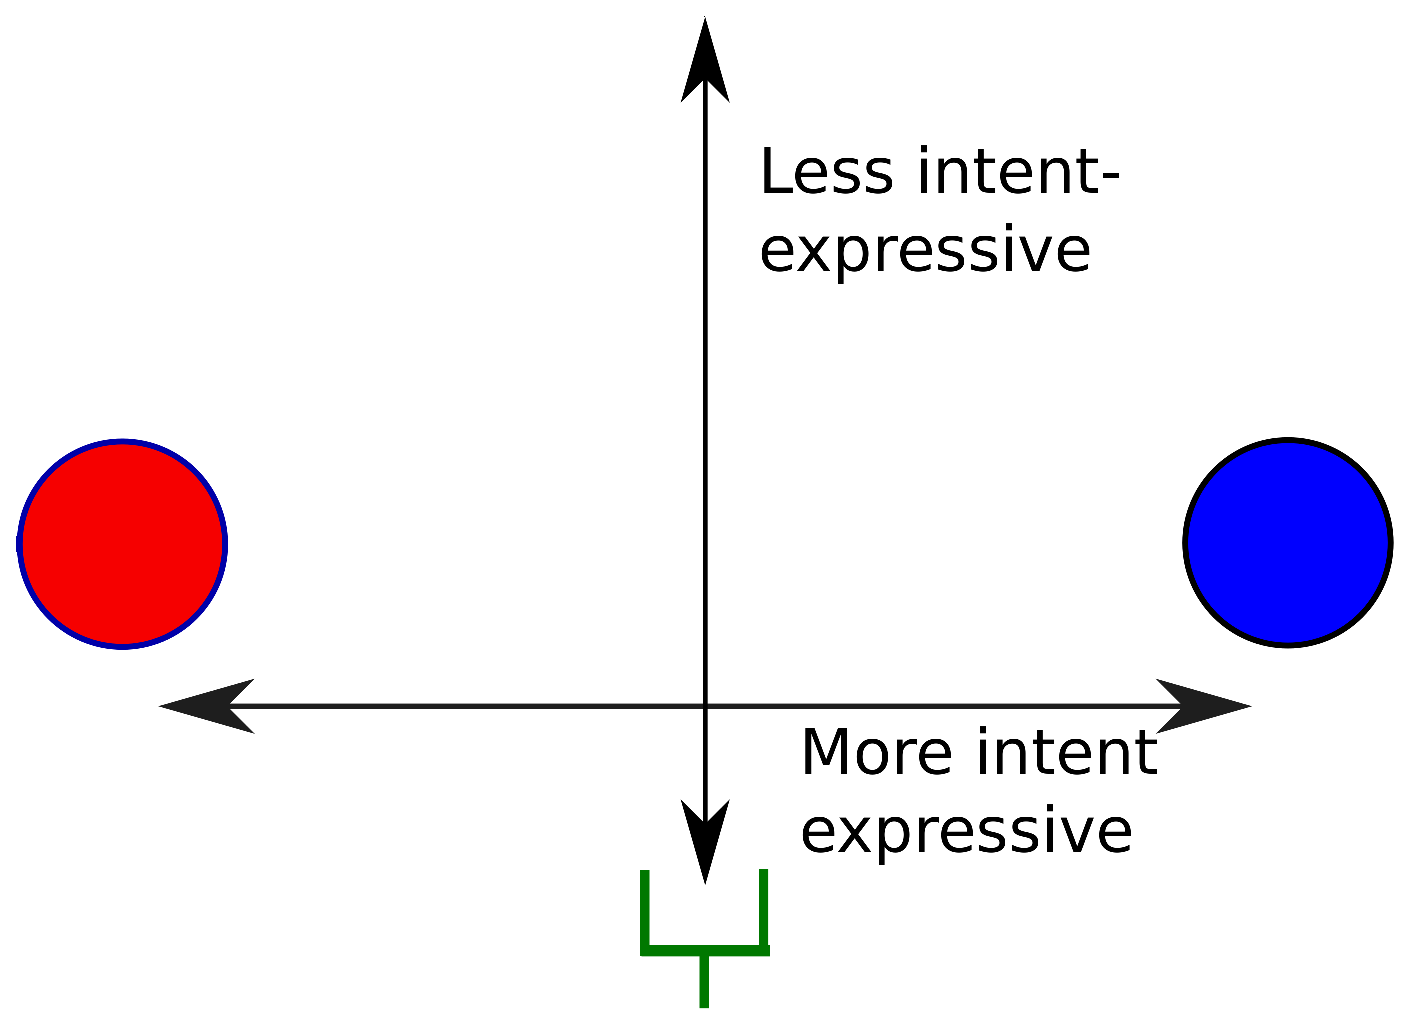
\includegraphics[width=0.35\textwidth]{./figures/Fig1_Disamb.eps}
	\end{center}
	%	\vspace{-.45cm}
	\caption{Illustration of goal disambiguation along various control dimensions. Any motion of the end effector (green) along the y-axis will not help the system to disambiguate the two goals (A and B). However, motion along the x-axis provides cues as to which goal.}
	\label{fig:disamb}
\end{figure}

In this work, as our primary contribution we develop a mode switch assistance paradigm that enhances the robot's intent inference capabilities, by selecting the control mode in which a user-initiated motion will \textit{maximally disambiguate} human intent. As depicted in the Figure~\ref{fig:shared_control} the intent disambiguation layer functions as a filter between the human commands and the intent inference engine. The disambiguation layer elicits more \textit{intent expressive} commands from the user by placing the user control is certain control modes. Furthermore, the disambiguation power of the algorithm is closely linked to, and is dependent on, the success and accuracy of the underlying intent inference mechanism. Therefore. as our secondary contribution, we also develop a novel intent inference scheme which utilizes ideas from \textit{dynamic field theory} that efficiently incorporates information contained in past history of states thereby ensuring the success of the disambiguation system. 
%More specifically on how well past cues are incorporated into the inference process.
\begin{figure*}[t!]
	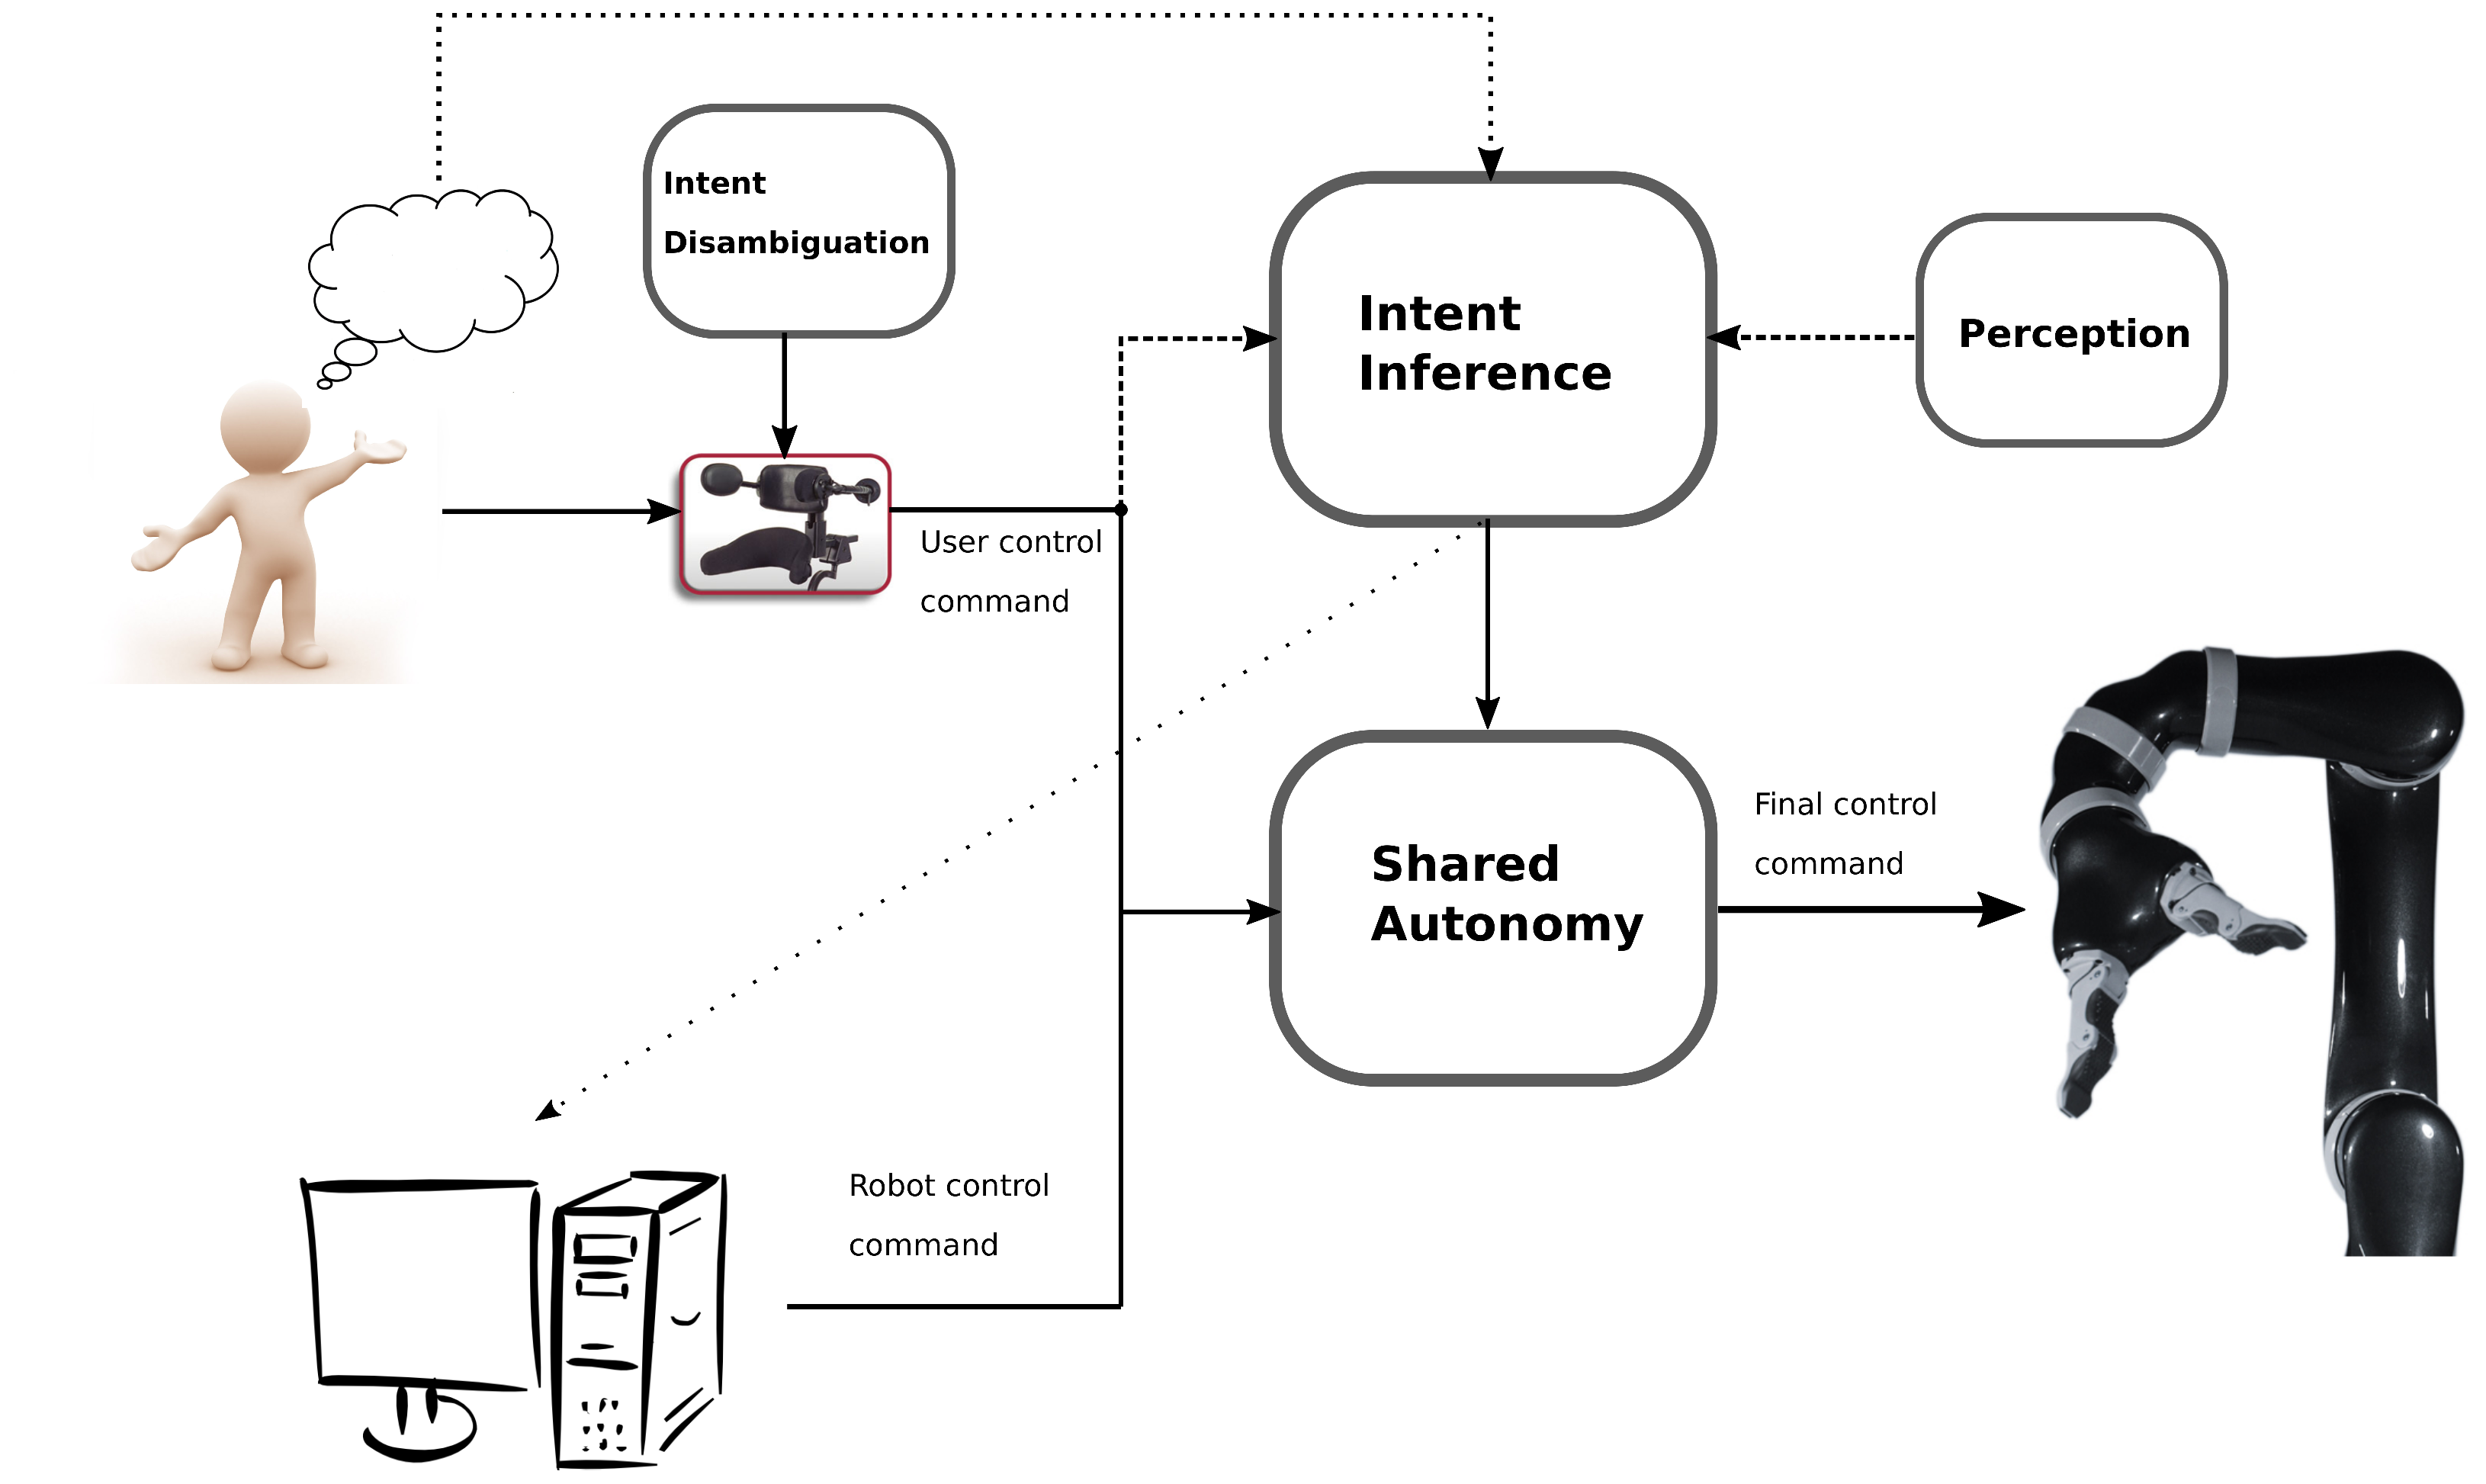
\includegraphics[keepaspectratio, width = \textwidth]{./figures/Fig2_SharedControl.eps}
	\caption{Core components of a Shared Control Architecture. }
	\label{fig:shared_control}
\end{figure*}
In Section~\ref{sec:related-work} we present a comprehensive overview of relevant research in the area of shared autonomy in assistive robotics, types of shared autonomy assistance paradigms, intent inference and synergies in human-robot interaction. Section~\ref{sec:ma} presents the mathematical formalism developed for intent inference and disambiguation and Section~\ref{sec:shared-control} focuses on the implementation details of the shared control system. The study design and experimental methods are discussed in Section~\ref{sec:ed} followed by results in Section~\ref{sec:results}. Discussions and conclusions are presented in Sections~\ref{sec:discussions} and~\ref{sec:conclusions} respectively. 


%%Understanding intent is critical. Why? Shared intention in human-human teams. Human-robot teams. Different types of paradigms exist for the same. 
%
%But we have human-in-th-loop. If the robot can elicit more intent expressive actions from the user, the inference problem becomes easier for the robot. Therefore the intent disambiguation system. 


\section{Related Work}\label{sec:related-work}
This section provides a comprehensive overview of related research in the domains of shared autonomy in assistive robotics, robot assistance for modal control, intent inference in human-robot interaction and information acquisition in robotics. 

Shared-autonomy in assistive systems aims to reduce user's cognitive and physical burden during task execution without having the user relinquish complete control~\cite{philips2007adaptive,demeester2008user, gopinath2017human, muelling2017autonomy}. Shared autonomy is preferred over fully autonomous robotic systems due to enhanced user satisfaction and robustness. The most common strategies to share control between the user and the assistive system include a) a hierarchical paradigm in which the higher level goals are entrusted with the user and the autonomy generates low-level control~\cite{tsui2011want, kim2010relationship, kim2012autonomy}, b) control allocation in distinct partitions of the entire control space~\cite{driessen2005collaborative} and c) blending user controls and robot autonomy commands~\cite{downey2016blending, storms2014blending, muelling2017autonomy}. 

In order to offset the drop in task performance due to shifting focus (\text{task switching}) from the task at hand to switching between different control modes different mode switch assistance paradigms have been proposed. Even a simple time-optimal mode switching scheme has shown to improve task performance~\cite{herlant2016assistive}. 
%Mode switch assistance schemes have also been proposed as a goal disambiguation mechanism which will help in improving the robot's intent inference capabilities~\cite{gopinath2017mode}. 
%~\cite{baker2007goal, baker2009action}
Shared control systems often require a good estimate of the humans' intent---for example, their intended reach target in a manipulation task or a target location in the environment in a navigation task~(\cite{liu2016goal}). Intent can either be explicitly communicated by the user~\cite{choi2008laser} or can be inferred using various algorithms from their control signals or sensor data. Intent recognition and inference are actively studied by cognitive scientists and roboticists and can be broadly categorized into two main classes: model-based approaches and heuristic approaches. In the model-based approach, intent inference is typically cast within the Bayesian framework, and the posterior distribution over goals (belief) at any time is determined by the iterative application of Bayes theorem. Evidence in this context can be derived from a combination of factors such as task-relevant features in the environmental, human control actions, biometric data from the user \textit{et cetera}. The user is modeled as a Partially Observable Markov Decision Process (POMDP) and is assumed to behave according to a predefined control policy that maps the states to actions. Although iterative belief updating using Bayes theorem provides an optimal strategy to combine new evidence (likelihood) with \textit{a priori} information (prior), incorporating an extended history of past states and control actions increases the computational complexity and tractability becomes an issue. In such cases,  first-order Markovian independence assumption makes the inference tractable. On the other hand, heuristic approaches are often simpler and seek to find direct mappings from instantaneous cues and the underlying human intention. For example, the use of instantaneous confidence functions for estimating intended reach target in robotic manipulation~\cite{dragan2012assistive, gopinath2017human}.  However, heuristic methods are not sophisticated enough to incorporate past histories of states and actions making them less robust to external noise resulting in erroneous inferences. 
%Although computationally simple, heuristic methods lack the sophistication to incorporate past histories of states resulting in erroneous inferences and is not robust enough to external noise. Heuristic methods are often computationally simple making it suitable for real-time applications.

Eliciting more legible and information-rich control commands from the user to improve intent estimation can be thought of as an information acquisition process. Intent estimation can be an \textit{active} process in which the robot takes actions that will probe the human's intent~\cite{sadigh2016information, sadigh2016planning}. Designing optimal control laws that maximizes information gain can be accomplished by having the associated reward structure reflect some measure of information gain~\cite{atanasov2014information}. 
Autonomous robots designed for exploration and data acquisition tasks can benefit from exploring more information-rich regions in the environment. If the spatial distribution of information density is known \textit{a priori}, information maximization can be accomplished by maximizing the ergodicity of the robot's trajectory with respect to the underlying information density map~\cite{miller2016ergodic, miller2013trajectory}. 

By having the humans assist the robot improve its intent inference capabilities, our work leverages the underlying synergies that are inherent in human-robot cooperation. In the context of human-human cooperative teams, the notion of shared intentionality---one in which all parties involved in a collaborative task team share the same intention/goal and have a joint commitment towards it---is crucial to make task execution more seamless and efficient~\cite{tomasello2007shared, tomasello2010gap}. This principle is relevant for successful human-robot interaction as well. From the robot's perspective, the core idea behind our disambiguation system is that of \textit{``Help Me, Help You''}---that is, if the user can help the robot with more information-rich actions, then the robot in turn can provide accurate and appropriate task assistance more quickly and confidently. A framework for \textit{``people helping robots helping people''} in which the robot relies on semantic information and judgments provided by the human to improve its own capabilities has been developed in ~\cite{sorokin2010people}. In order to overcome the various types of communication bottlenecks that can hamper performance, different types of communication interfaces have been developed that account for the restricted capabilities of the robot~\cite{goodfellow2010help}. Lastly, more intent-expressive actions \textit{by} the human is closely related to \textit{legibility} of motions. In HRI, the legibility and predictability of robot motion \textit{to} the human has been investigated~\cite{dragan2013legibility} and various techniques to generate legible robot motion have been proposed as well~\cite{holladay2014legible}. We rely on the idea of \textit{inverse legibility}~\cite{gopinath2017mode} in which the assistance scheme is intended to bring out more legible intent-expressive control commands \textit{from} the human. 
\section{Mathematical Formalism}\label{sec:ma}
%\subsection{Subsection title}\label{sec:2}
%as required. Don't forget to give each section
%and subsection a unique label (see Sect.~\ref{sec:1}).
This section describes our intent disambiguation algorithm that computes the control mode that can maximally disambiguate between the goals and the intent inference mechanism that works in conjunction with the disambiguation algorithm. Section~\ref{ssec:notation} outlines the mathematical notation used in this paper. Section ~\ref{ssec:disamb} describes the disambiguation algorithm. The mathematical details of the intent inference paradigms is outline in detail in Section~\ref{ssec:inference}.
% Section~\ref{sec:shared-control} describes the blending-based shared control system implemented in our work. 
\subsection{Notation}\label{ssec:notation}
Let $\mathcal{G}$ denote the set of all candidate goals with $n_g = \vert\mathcal{G}\vert$ and let $g^i$ refer to the $i^{th}$ goal with $i \in [1,2,\dots, n_g]$. A \textit{goal} represents the human's underlying intent. Specifically, in assistive robotic manipulation, since the robotic device is primarily used for reaching toward and grasping of discrete objects in the environment, intent inference is the estimation of the probability distribution over all possible goals (objects) in the environment. At any time $t$, the robot actively maintains a probability distribution over goals denoted by $\boldsymbol{p}(t)$ such that $\boldsymbol{p}(t) = [p^1(t), p^2(t),\dots, p^{n_g}(t)]^{T}$ where $p^i(t)$ denotes the probability associated with goal $g^i$.  The probability $p^i(t)$ represent the robot's \textit{confidence} that goal $g^i$ is the human's intended goal. 

Let $\mathcal{K}$ be the set of all controllable dimensions of the robot and $k^i$ represent the $i^{th}$ control dimension where $i \in [1,2,\dots,n_k]$. The cardinality of $\mathcal{K}$ is denoted as $n_k$ and typically depends on the robotic platform used. For example, for a smart wheelchair $n_k = 2$, since the controllable degrees-of-freedom are velocity and heading and for a six degrees-of-freedom robotic arm with a gripper $n_k = 7$. 

The limitations of the control interfaces necessitate the control space $\mathcal{K}$ to be partitioned into control modes. Let $\mathcal{M}$ denote the set of all control modes with $n_m = \vert\mathcal{M}\vert$. Additionally, let $m^i$ refer to the $i^{th}$ control mode where $i \in [1,2,\dots,n_m]$. Each control mode $m^i$ is a subset of $\mathcal{K}$ such that $\bigcup\limits_{i=1}^{n_m} m^i$ spans all of the controllable dimensions. Let $\boldsymbol{e}^i$ be the standard basis vectors that denote the unit velocity vector along the $i^{th}$ control dimension\footnote{For the rotational control dimensions, the velocity is specified with respect to the end-effector of the robotic frame.}. The disambiguation formalism developed in Section~\ref{ssec:disamb} is agnostic to the particular form of intent inference. However, the algorithm assumes that $\boldsymbol{p}(t)$ can be forward projected in time by iteratively applying the intent inference algorithm. 

The disambiguation metric that characterizes the disambiguation capabilities of a control dimension $k \in \mathcal{K}$ is denoted by $D_k \in \mathbb{R}$. We explicitly define disambiguation metrics for both positive negative motions along $k$ as $D_k^{+}$ and $D_k^{-}$ respectively. We also define a disambiguation metric $D_m \in \mathbb{R}$ for each control mode $m \in \mathcal{M}$. $D_m$ is a measure of how informative and useful the user control commands would be for the robot if the user were to operate the robot in control mode $m$. The higher it is, the easier it will be for the system to infer human's intent. Both $D_k$ and $D_m$ will be formally defined in Section~\ref{sssec:components}.

The robot pose and the goal pose for $g \in \mathcal{G}$ are denoted $\boldsymbol{x}_r$ and $\boldsymbol{x}_g$ respectively and $\boldsymbol{u}_h$ denotes the human control command.
\subsection{Intent Disambiguation}\label{ssec:disamb} 
The need for intent disambiguation arises from how the probability distribution over goals evolves as the user controls the robot and moves it in space. That is, given an intent inference mechanism that is dependent on robot pose or movement (\textbf{cite TODO, refer notes}), as the user controls the robot in different control modes, the probability distribution evolves. Figure~\ref{fig:disamb_motivation} shows simulations which motivate the development of a disambiguation metric. For different control modes, the confidences associated with each goal are different. Moreover, motions in some control modes result in sharper rise in some goal confidences compared to others. This indicates the existence of control modes that can better disambiguate between the goals. 

\begin{figure}[h]
	\centering
	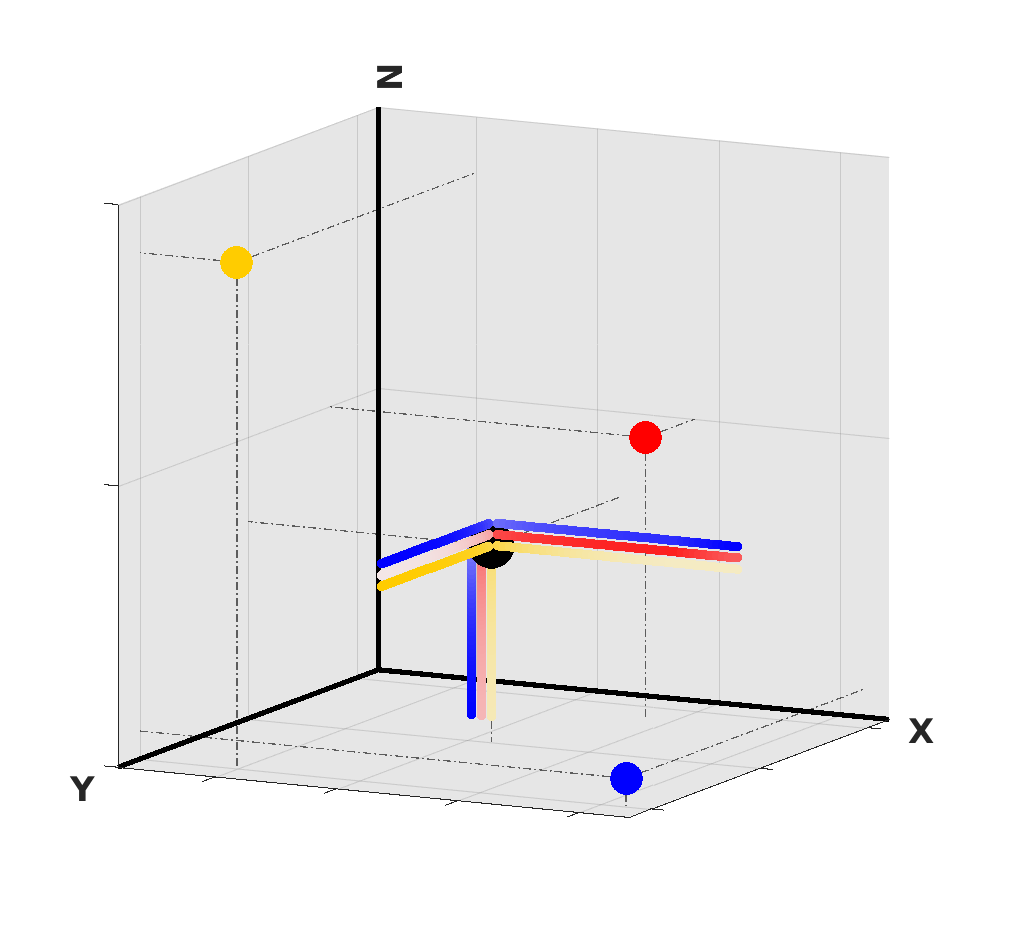
\includegraphics[width = 1\hsize]{./figures/disamb_motivation_new_origin_new_goals.eps}
	%	\vspace{-0.35cm}
	\caption{Illustration of how goal confidences change upon motion along control dimensions. The three colored lines along each dimension represent the confidences associated with a goal of corresponding color. One can see that motion along certain control dimensions result in sharper rise in confidences for some goals compared to others.}
	\label{fig:disamb_motivation}
\end{figure}
The computation of $D_k$ depends on four components (denoted as $\Gamma_k$, $\Omega_k$, $\Lambda_k$ and $\Upsilon_k$), which in turn depend on a projection of the probability distribution over intent. These computations and projection are described in detail in Section~\ref{sssec:projection} and Section~\ref{sssec:components}, and as a pseudocode in Algorithm~\ref{alg1}. 
%$D_k$ characterizes the disambiguation capabilities of a control dimension. The metric encodes different aspects of the probability distributions over goals upon moving along control dimension $k$. 

\subsubsection{Forward Projection of $\boldsymbol{p}(t)$}\label{sssec:projection}
The first step towards the computation of $D_k$ is the forward projection of the probability distribution $\boldsymbol{p}(t)$ from the current time $t_a$ to $t_b$ and $t_c$ ($t_a < t_b < t_c$), Algorithm~\ref{alg1}, lines 3-13). Application of control command $\boldsymbol{e}^k$ results in probability distributions $\boldsymbol{p}^+_k(t_b)$, $\boldsymbol{p}^+_k(t_c)$ and $-\boldsymbol{e}^k$ results in $\boldsymbol{p}^-_k(t_b)$ and $\boldsymbol{p}^-_k(t_c)$. Not that Algorithm~\ref{alg1} is run twice, to compute the projected probability distributions for $\boldsymbol{e}^k$ and $-\boldsymbol{e}^k$.

 The exact computation of the projected probability distribution will depend on the underlying intent inference computation---for example, whether it depends on $\boldsymbol{x_r}$ (which can be computed from $\boldsymbol{e}^k$ applied to the robot kinematics model) or $\boldsymbol{u}_h$ (which can be taken as $\boldsymbol{e}^k$). All parameters and features which affect the computation of $\boldsymbol{p}(t)$ are denoted as $\boldsymbol{\Theta}$. 

%\footnote{Going forward, for the sake of brevity, $t+\Delta t$ and $t + 2 \Delta t$ will be denoted as $\delta t$ and $\delta\delta t$ from}
%Four important characteristics (denoted by $\Gamma_k$, $\Omega_k$, $\Lambda_k$ and $\Upsilon_k$) of the projected probability distributions are then combined to compute the disambiguation metric $D_k$. The computation of each of these characteristics is described in Section~\ref{sssec:components}. The pseudo-algorithm for forward projection of $\boldsymbol{p}(t)$ and computation of $D_k$ is outlined in Algorithm~\ref{alg1}.
% Note that the algorithm is used twice to compute the projected probability distributions for $\boldsymbol{e}^k$ and $-\boldsymbol{e}^k$\footnote{The \textit{UpdateIntent} function used in the algorithm is described in detail in Section~\ref{sssec:dft_ii}.}. The kinematic model works in the full translation and orientation space. 
\begin{algorithm}
	\caption{Calculate $\boldsymbol{p}(t_b)$, $\boldsymbol{p}(t_c)$}
	\label{alg1}
	\begin{algorithmic}[1]
		\REQUIRE $\boldsymbol{p}(t_a), \boldsymbol{x}_r(t_a), \Delta t, t_a < t_b < t_c, \boldsymbol{\Theta}$
%		\ENSURE $t_c > t_b > t_a$
		\FOR{$k=0\dots n_k$}
		\STATE Initialize $D_k = 0$, $t = t_a$
		
%		\STATE $D_k \leftarrow 0,D_k^+ \leftarrow 0, D_k^- \leftarrow 0 $
%		\STATE $t \leftarrow t_a$
%		\STATE $\boldsymbol{p}_k^+(t) \leftarrow \boldsymbol{p}(t_a)$; 
%		\STATE $\boldsymbol{x}_r^+(t) \leftarrow \boldsymbol{x}_r(t_a)$; 
%		\STATE $\boldsymbol{u}_h^+ \leftarrow \boldsymbol{e}^k$;
		\WHILE{$t \leq t_c$}
%		\FOR {$t = t_a\dots t_c$}
			\STATE $\boldsymbol{p}_k(t + \Delta t) \leftarrow \text{UpdateIntent}(\boldsymbol{p}_k(t), \boldsymbol{u}_h; \boldsymbol{\Theta})$
			\STATE $\boldsymbol{x}_r(t + \Delta t) \leftarrow \text{SimulateKinematics}(\boldsymbol{x}_r(t), \boldsymbol{u}_h)$
			\IF{$t = t_b$} \STATE {$Compute \;\;\Gamma_k, \Omega_k, \Lambda_k$} 
			\ENDIF
			\IF{$t = t_c$} \STATE{$Compute \;\;\Upsilon_k$} \ENDIF
			\STATE $t \leftarrow t + \Delta t$
%		\ENDFOR
%		\WHILE{$ t \leq t_c$}
		\ENDWHILE
	
%		\STATE $\boldsymbol{p}^-_k(t + \Delta t) \leftarrow UpdateIntent(\boldsymbol{p}^-_k(t), \boldsymbol{u}_h^-; \boldsymbol{\Theta})$
%		\STATE $\boldsymbol{x}_r^-(t + \Delta t) \leftarrow SimulateDynamics(\boldsymbol{x}_r^-(t), \boldsymbol{u}_h^-)$
%		
		
%		\ENDWHILE
		\STATE $Compute \;\;D_k$
		\ENDFOR
		
	\end{algorithmic}
\end{algorithm}

\subsubsection{Components of $D_k$}\label{sssec:components}
The computation of disambiguation metric $D_k$ consists of four components. Each of the following components encodes some aspect of the shape of the probability distribution and is computed for projections along both positive and negative directions independently. The four components are computed in lines 7 and 10 in Algorithm~\ref{alg1}.

1) \textit{Maximum probability:} The maximum of the projected probability distribution $\boldsymbol{p}_k(t_b)$  is a good measure of the robot's overall certainty in accurate predicting human intent (The maximum of this discrete probability distribution is the mode of the distribution). A higher value implies that the robot has a good idea of which goal is the humans's intended goal. We define the distribution maximum as $\Gamma_k$.
\begin{equation}
\Gamma_k = \max\limits_{1 \leq i \leq n_g}p^i_k(t_b)
\end{equation}

2) \textit{Difference between largest probabilities:} Disambiguation accuracy benefits from greater differences between the first and second most probable goals. This difference is denoted as $\Omega_k$.
\begin{equation}
\Omega_k = \text{max}(\boldsymbol{p}_k(t_b)) - \text{max}(\boldsymbol{p}_k(t_b) \setminus \text{max}(\boldsymbol{p}_k(t_b)))
\end{equation}

3) \textit{Pairwise separation of probabilities:} If the difference between the largest probabilities fails to disambiguate, then the separation, $\Lambda_k$, in the remaining goal probabilities will further aid in intent disambiguation. The quantity $\Lambda_k$ is computed as the \textit{sum of the pairwise distances} between the $n_g$ probabilities.
\begin{equation}
\Lambda_k = \sum_{i=1}^{n_g}\sum_{j=i}^{n_g}\lvert p^i_k(t_b) - p^j_k(t_b)\rvert
\end{equation}
\begin{figure*}[t]
	\centering
	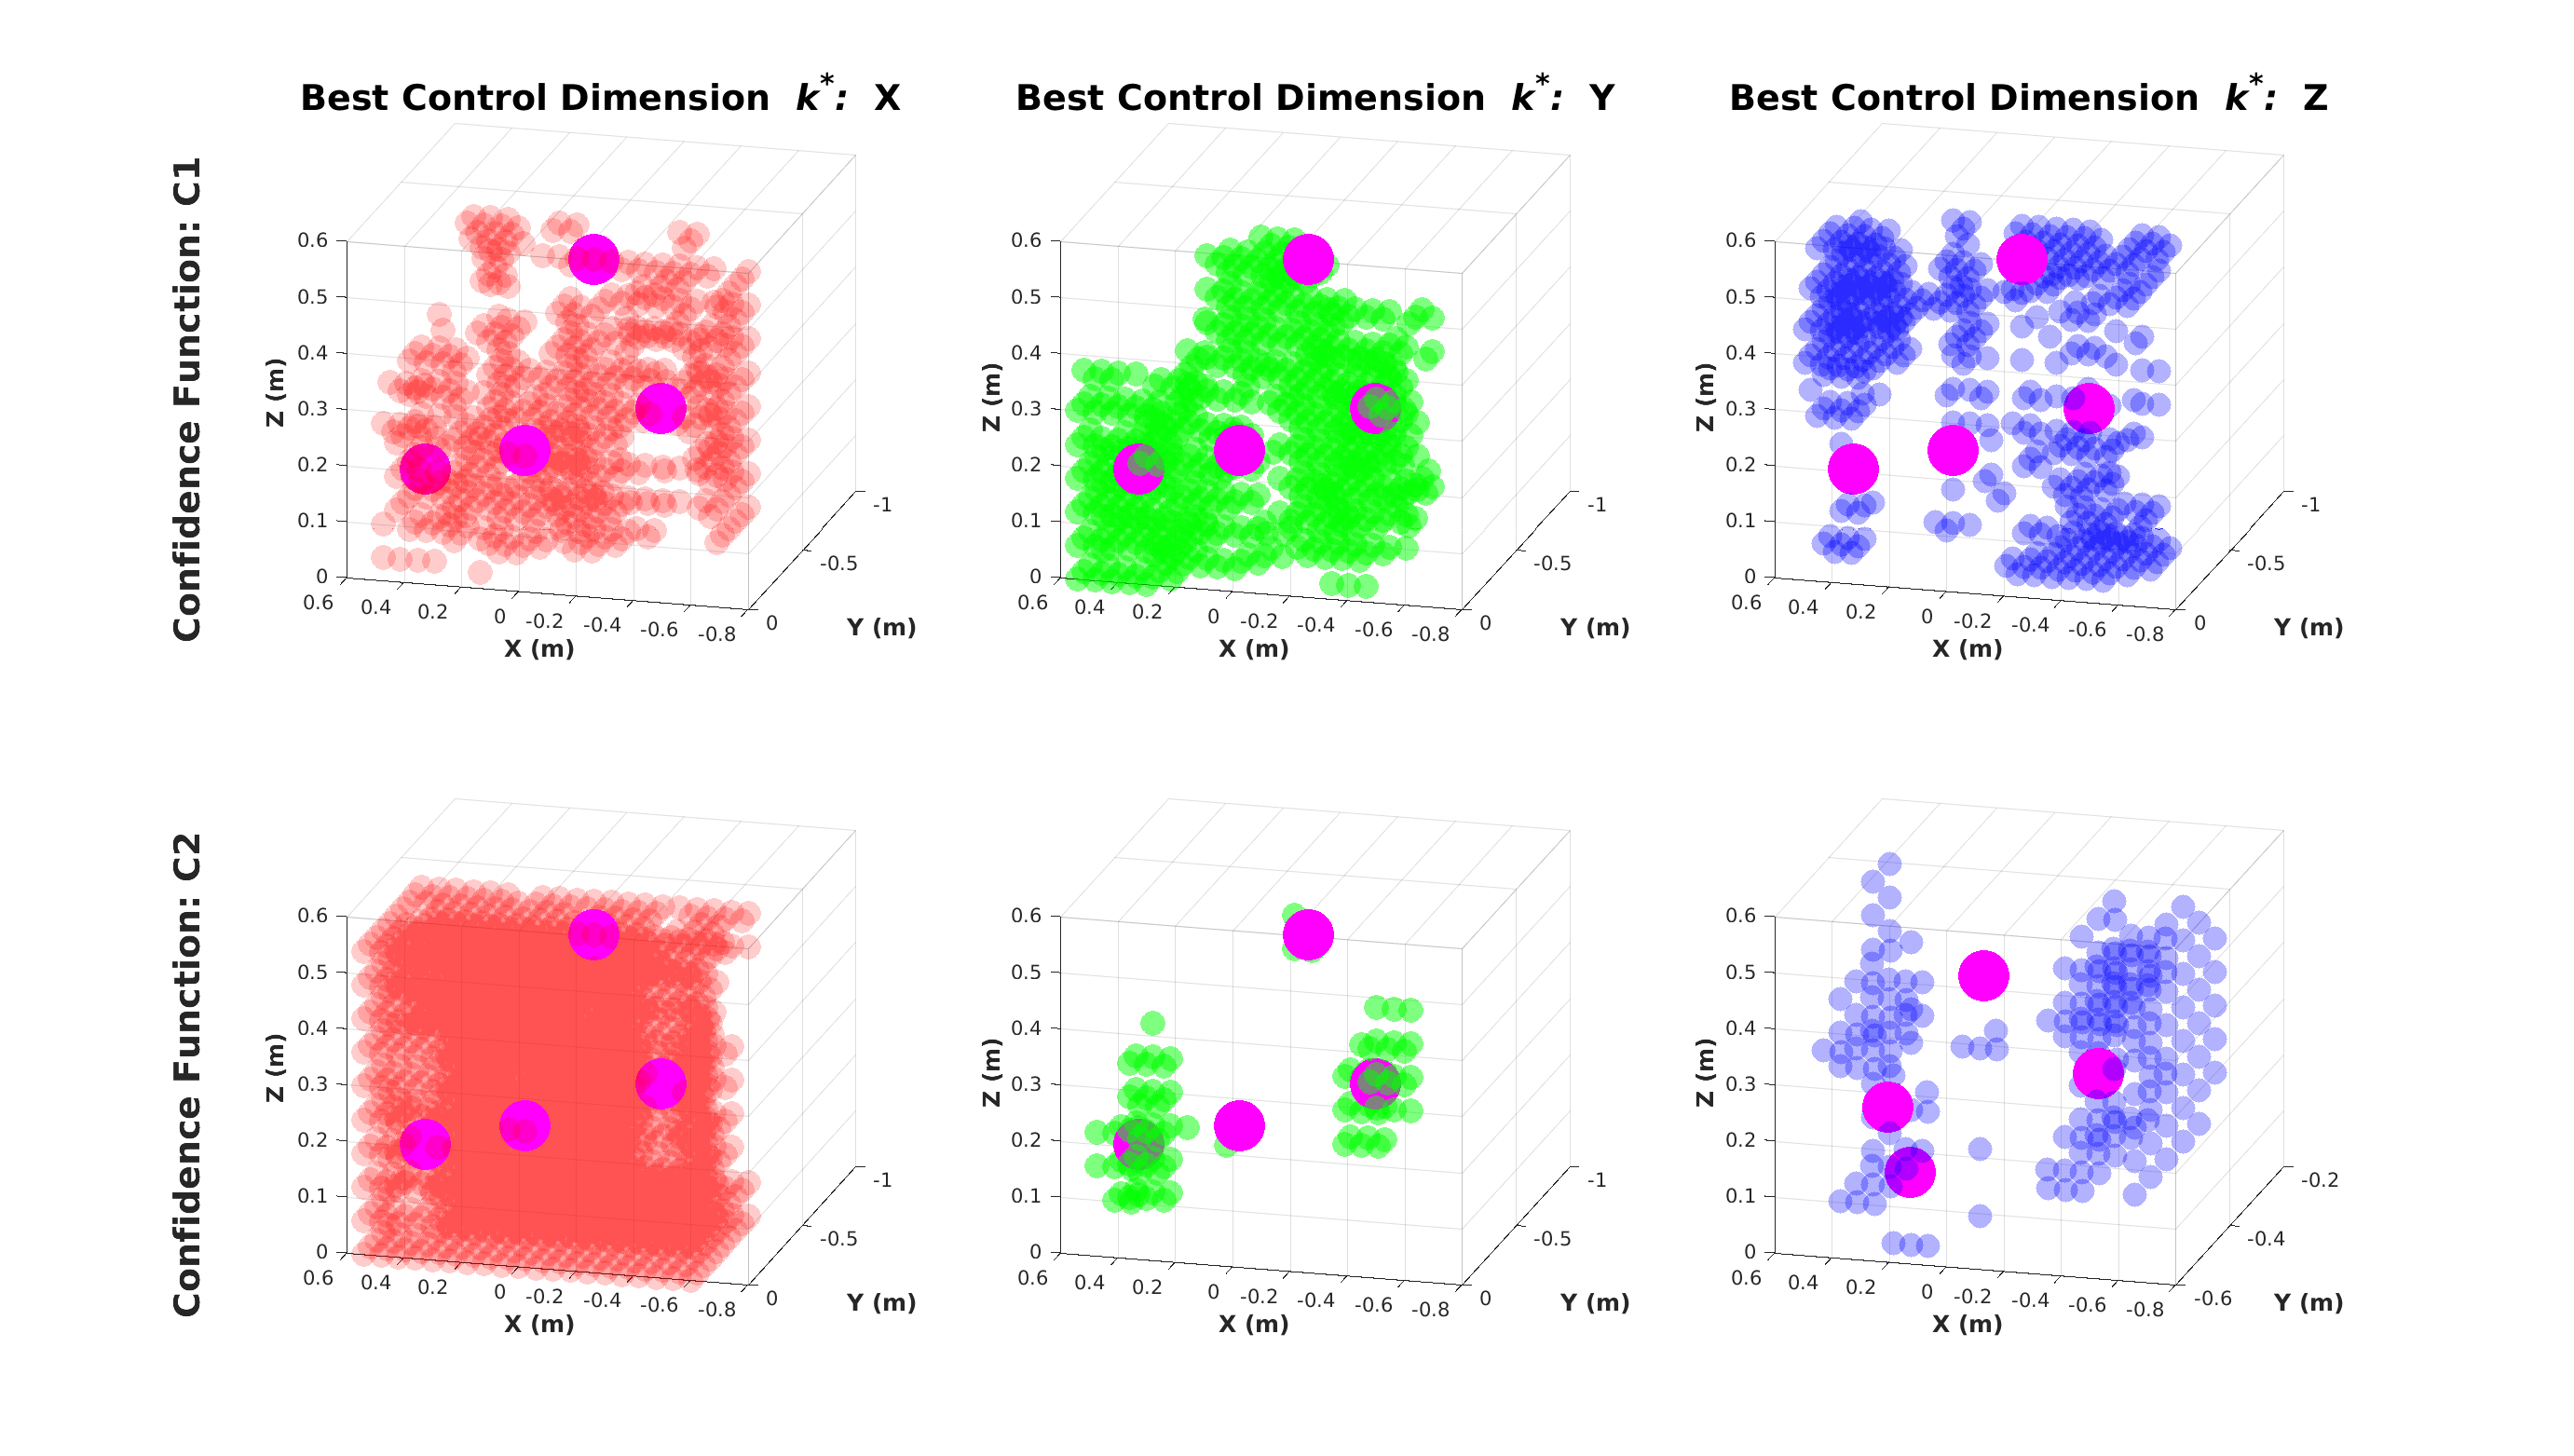
\includegraphics[width = 1.15\hsize, height = 0.6\vsize, center]{./figures/sim_res.eps}
	\caption{Control dimensions best able to disambiguate intent.  Left column: $k^*$ is X. Middle Column: $k^*$ is Y. Right Column: $k^*$ is Z. Magenta spheres indicate the goal locations (intent). In this example, the goals are spread maximally along the x and z dimensions, and so inference happens more quickly if the human control commands are along x or z. We see that x and z are chosen more often as the most disambiguating dimensions when using intent inference function \textbf{C2} (bottom row). Function \textbf{C2} considers the instantaneous directedness of the human's control command towards that goal, while inference function \textbf{C1} (top row) encodes only proximity to a given goal. Function \textbf{C2} is considered to encode more information about the human's intent than \textbf{C1}, with the result of stronger inference power---which is inherently linked to the disambiguation power of our algorithm. Further details in~\cite{gopinath2017mode}.}
	\label{fig:sim_res}
\end{figure*}
4) \textit{Gradients:} The probability distribution $\boldsymbol{p}_k(t)$ can undergo drastic changes upon continuation of motion along control dimension $k$. The spatial gradient of $\boldsymbol{p}_k(t)$ encodes this propensity for change and is approximated by 
\begin{equation}
\frac{\partial\boldsymbol{p}_k(t)}{\partial x_k} = \boldsymbol{p}_k(t_c) - \boldsymbol{p}_k(t_b)
\end{equation}
where $x_k$ is the component of robot's displacement along control dimension $k$. The greater the difference between individual spatial gradients, the greater will the probabilities deviate from each other, thereby helping in disambiguation. In order to quantify the ``spread'' of gradients we define a quantity $\Upsilon_k$ 
\begin{equation}
\Upsilon_k = \sum_{i=1}^{n_g}\sum_{j=i}^{n_g}\Big \lvert\frac{\partial p^i_k(t)}{\partial x_k} - \frac{\partial p^j_k(t)}{\partial x_k}\Big \rvert
\end{equation}
where $\lvert\cdot\rvert$ denotes the absolute value. 
\textit{Putting it all together:}
$\Gamma_k$, $\Omega_k$, $\Lambda_k$ and $\Upsilon_k$ are then combined to compute $D_{k}$ as 
\begin{equation}\label{DK}
D_{k} = \underbrace{w\cdot(\Gamma_k\cdot \Omega_k\cdot\Lambda_k)}_{\text{short-term}} + \underbrace{(1 - w)\cdot \Upsilon_k}_{\text{long-term}}
\end{equation}

where $w$ is a task-specific weight that balances the contributions of the short-term and long-term components. (In our implementation, $w=0.5$.) Equation~\ref{DK} actually is computed twice, once in each of the positive ($\boldsymbol{e}^k$) and negative directions ($-\boldsymbol{e}^k$) along $k$, and the results ($D_k^+$ and $D_k^-$) are then summed. The computation of $D_k$ is performed for each control dimension $k \in \mathcal{K}$. The disambiguation metric $D_m$ for control mode $m$ then is calculated as 
\begin{equation}\label{EQ2}
D_m = \sum_{k} D_{k} \;
\end{equation}
where $k \in m$ iterates through the set of control dimensions on which $m$ is able to operate.
Lastly, the control mode with highest disambiguation capability $m^*$ is given by
\begin{equation*}
m^* = \argmax_m  D_{m}
\end{equation*}
while $k^* = \argmax_k D_k$ gives the control dimension with highest disambiguation capability $k^{*}$.
%\begin{equation*}
%k^* = \argmax_k D_k~~~.
%\end{equation*}
Disambiguation mode $m^{*}$ is the mode that the algorithm chooses \textit{for} the human to better estimate their intent. Any control command issued by the user in $m^*$ is likely to be more useful for the robot in determining which is the human's intended goal, because of the maximal confidence disambiguation.

\subsection{Intent Inference}\label{ssec:inference}
This section describes the intent inference scheme used in this paper. Our preliminary work~\cite{gopinath2017mode} revealed that the power of our disambiguation algorithm proposed in Section~\ref{ssec:disamb} is intimately linked with the inference power of different choices of intent inference mechanisms. More importantly, the pilot study associated with this preliminary work suggested that incorporating a history of past states and actions would improve performance. We therefore propose an extended disambiguation formulation which furthermore incorporates history.
% Intent inference using Bayesian approaches theoretically can take into account the influence of past history; however due to computational expenses low-order Markovian assumptions are usually made to make the inference tractable. 

In this work, we propose a novel intent inference scheme inspired by \textit{dynamic field theory} in which the time evolution of the probability distribution $\boldsymbol{p}(t)$ is specified as a dynamical system with constraints. An alternate approach is to perform intent inference using Bayesian techniques, which in theory can take into account the influence of past states and actions. In practice, however, low-order Markov assumptions are usually made to make the inference tractable computationally, and with such assumptions history is lost.

 Section~\ref{sssec:dft} provides a primer on the basic principles and features of \textit{dynamic field theory} and its application in the fields of neuroscience and cognitive robotics. Section~\ref{sssec:dft_ii} describes our novel formulation that makes use of dynamic field theory for the purposes of intent inference. 

\subsubsection{Dynamic Field Theory}\label{sssec:dft}

In Dynamic Field Theory (DFT)~\cite{schoner2015dynamic}, variables of interest are treated as dynamical state variables. To represent the information about these variables requires two dimensions: one which specifies the value the variables can attain (the domain) and the other which encodes the \textit{activation level} or the amount of information about that a particular value. These \textit{activation fields} are analogous to probability distributions defined over a random variable. 

%In DFT the dynamical system that specifies the temporal evolution of activation fields is constrained by the postulate that localized peaks in the distribution are fixed point attractors, or in other words \textit{stable}.
Following Amari's formulation~\cite{amari1977dynamics} dynamics of an activation field $\phi(x, t)$ are given by 
\begin{multline}
\tau\dot{\phi}(x,t) = -\phi(x,t) + h + S(x,t) + \\ \int\limits_{}^{}dx^{\prime}b(x-x^{\prime})\sigma(\phi(x^{\prime}, t)) 
\end{multline} 
where $x$ denotes the variable of interest, $t$ is time, $\tau$ is the time-scale parameter, $h$ is the constant resting level, and $S(x,t)$ is the external input, $b(x-x^\prime)$ is the interaction kernel and $\sigma(\phi)$ is a sigmoidal nonlinear threshold function. The interaction kernel mediates how activations at all other field sites $x^\prime$ drive the activation level at $x$. Two types of interactions are possible: excitatory (when interaction is positive) which drives up the activation, and inhibitory (when the interaction is negative) which drives the activation down. 
Historically, dynamic neural fields originally were conceived to explain cortical population neuronal dynamics, based on the hypothesis that the excitatory and inhibitory neural interactions between local neuronal pools form the basis of cortical information processing~\cite{wilson1973mathematical}. 

Dynamic neural fields possess some unique characteristics that make them ideal candidates for modeling higher-level cognition. First, a peak in the activation field can be \textit{sustained} even in the absence of external input due to the recurrent interaction terms. Second, information from the past can be \textit{preserved} over much larger time scales quite easily by tuning the time-scale parameter thereby endowing the fields with memory. Third, the activation fields are \textit{robust} to disturbance and noise in the external output~\cite{schoner2008dynamical}. 
As a result, DFT principles have found widespread application in the area of cognitive robotics~\cite{erlhagen2006dynamic}, specifically in the contexts of efficient human-robot interaction~\cite{erlhagen2014dynamic}, robotic scene representation~\cite{zibner2011dynamic}, obstacle avoidance and target reaching behaviors in both humans and robots~\cite{schoner1995dynamics}, and for object learning and recognition~\cite{faubel2008learning}. 


\subsubsection{Dynamic Neural Fields for Intent Inference}\label{sssec:dft_ii}

Recurrent interaction between the state variables, 
robustness to noise and inherent memory make dynamic neural fields an ideal candidate for an intent inference engine. Our insight is to use the framework of dynamic neural fields to specify the time evolution of the probability distribution $\boldsymbol{p}(t)$, in which we treat the individual goal probabilities $p^i(t)$ as constrained dynamical state variables such that $p^i(t) \in [0, 1]$ and $\Sigma_{1}^{n_g}p^{i}(t) = 1$. The dynamical system can be generically written as 
\begin{equation}
\dot{\boldsymbol{p}}(t) = F(\boldsymbol{p}(t), \boldsymbol{u}_h ; \boldsymbol{\Theta})
\end{equation}
where $F$ represents the nonlinear vector field, $\boldsymbol{u}_h$ is the human control input and $\boldsymbol{\Theta}$ represents all other task-relevant features and parameters that affect the time-evolution of the probability distribution. 
The full specification of the neural field is given by
\begin{multline}\label{eq:dft}
\frac{\partial \boldsymbol{p}(t)}{\partial t} = \frac{1}{\tau}\bigg[-\mathbb{I}_{n_g\times n_g}\cdot\boldsymbol{p}(t) + \underbrace{\frac{1}{n_g}\cdot\mathbbm{1}_{n_g}\bigg]}_{\text{rest state}} + \\ \underbrace{\boldsymbol{\lambda}_{n_g\times n_g}\cdot\sigma(\boldsymbol{z}(\boldsymbol{u}_h;\boldsymbol{\Theta}))}_{\text{excitatory + inhibitory}}
\end{multline}
where time-scale parameter $\tau$ which determines the memory capacity of the system, $\mathbb{I}$ is the identity matrix, $\boldsymbol{\lambda}$ is the control matrix that controls the excitatory and inhibitory aspects, $\boldsymbol{z}$ is a function that encodes the nonlinearity through which human control commands and task features affect the time evolution, and $\sigma$ is a biased sigmoidal nonlinearity given by $\sigma(\boldsymbol{z}) = \frac{1}{1 + e^{-\boldsymbol{z}}} - 0.5$.
The off-diagonal elements of $\boldsymbol{\lambda}$ mediate the interaction between all of the probabilities. In the absence of any information or cues, the probability distribution settles to a resting state which is a uniform distribution, that is whenever $\boldsymbol{u}_h = 0$, $\boldsymbol{z} = \vec{0}$. Given the initial probability distribution at time $t_a$ Equation~\ref{eq:dft} can be solved numerically from $t \in [t_a, t_b]$ using a simple Euler algorithm with a fixed time-step $\Delta t$.

The design of $\boldsymbol{z}$ is informed by what features of the human control input and environment capture the human's underlying intent most effectively. We rely on the \textit{directedness} of the human control commands towards a goal, the \textit{proximity} to a goal and the \textit{agreement} between the human commands and robot autonomy. 
With $\boldsymbol{\Theta} = \{\boldsymbol{x}_r, \boldsymbol{x}_{g^i}, \boldsymbol{u}_{r, g^i}\}$, one dimension $i$ of $\boldsymbol{z}$ is defined as 
\begin{multline}
z^i(\boldsymbol{u}_h;\boldsymbol{x}_r, \boldsymbol{x}_{g^i}, \boldsymbol{u}_{r, g^i}) = \underbrace{\frac{1 + \eta}{2}}_{\text{directedness}} + \underbrace{\boldsymbol{u}_{h}^{rot}\cdot\boldsymbol{u}_{r,g^i}^{rot}}_{\text{agreement}}
\\+ \underbrace{\text{max}\Big(0, 1-\frac{\norm{\boldsymbol{x}_{g^i} - \boldsymbol{x}_r}}{R}\Big)}_{\text{proximity}}
\end{multline}
where  $\eta = \frac{\boldsymbol{u}_h^{trans}\cdot(\boldsymbol{x}_{g^i} - \boldsymbol{x}_r)^{trans}}{\norm{\boldsymbol{u}_h^{trans}}\norm{(\boldsymbol{x}_{g^i} - \boldsymbol{x}_r)^{trans}}}$, $\boldsymbol{u}_{r,g^i}$ is the robot autonomy command for reaching goal $g^i$, $trans$ and $rot$ refer to the translational and rotational components of a command $\boldsymbol{u}$ or position $\boldsymbol{x}$,  $R$ is the radius of the sphere beyond which the proximity component is always zero, and $\norm{\cdot}$ is the Euclidean norm. That is, in the absence of any human control command, the probability distribution decays to the resting state which is a uniform distribution.  
%$cos(\eta) =  \frac{\boldsymbol{u}_h^{trans}\cdot(\boldsymbol{x}_{g^i} - \boldsymbol{x}_r)^{trans}}{\norm{\boldsymbol{u}_h\cdot\norm{\boldsymbol{x}_{g^i} - \boldsymbol{x}_r}}$, $\boldsymbol{u}_{r, g^i}$
The most confident goal $g^*$ then is computed as 
\begin{equation}
g^* = \argmax_i  p^i(t)
\end{equation}

At every time step the constraints on $p^i(t)$ are enforced thereby ensuring that $\boldsymbol{p}(t)$ is a valid probability distribution at all times. 
	
\section{Shared Control}\label{sec:shared-control}
The shared control paradigm implemented in our robot is a blending-based system in  which the final control command issued to the robot is a blended sum of the human control command and an autonomous robot policy.
The robot policy is generated by a function $f_{r}(\cdot) \in \mathcal{F}_{r}$, 
\begin{equation*}
\boldsymbol{u}_r \leftarrow f_{r}(\boldsymbol{x})
\end{equation*}
where $\mathcal{F}_{r}$ is the set of all control behaviors corresponding to different tasks. This set could be derived using a variety of techniques such as \textit{Learning from Demonstrations}~\cite{argall2009survey, schaal1997learning, khansari2011learning, calinon2012statistical}, motion planners~\cite{hsu2002randomized,ratliff2009chomp} and navigation functions~\cite{rimon1992exact,tanner2003nonholonomic}. Specifically, let $\boldsymbol{u}_{r,g}$ be the autonomous control policy associated with goal $g$. The final control command $\boldsymbol{u}$, issued to the robot then is given as 
\begin{equation*}
\boldsymbol{u} = \alpha\cdot \boldsymbol{u}_{r,g^*} + (1 - \alpha)\cdot \boldsymbol{u}_h
\end{equation*}
where $g^*$ is the most confident goal. The blending factor $\alpha$ is a piecewise linear function of the probability associated with $g^*$ denoted as $p(g^*)$ and is given by
$$
\alpha = \left\{
\begin{array}{ll}
0 & \quad p(g^*) \leq \theta_1 \\
\frac{\theta_3}{\theta_2 - \theta_1}\cdot p(g^*) &  \quad \theta_1 < p(g^*) \leq \theta_2  \\
\theta_3 & \quad p(g^*) > \theta_2 	
\end{array}
\right.
$$
with $\theta_i \in [0, 1] \;\forall\; i \in [1,2,3]$ and $ \theta_2 > \theta_1$. 
For effective shared control, we set $\theta_1 = \frac{1.2}{n_g}, \theta_2 = \frac{1.4}{n_g}$ and $ \theta_3 = 0.7$.

The robot control command $\boldsymbol{u}_{r,g}$ is generated using a simple potential field which is defined in all parts of the state space~\cite{khatib1986real}. Every goal $g$ is associated with a potential field $P_g$ which treats $g$ as an attractor and all the other goals in the scene as repellers. For potential field $P_g$, the attractor velocity is given by
\begin{equation*}
\dot{\boldsymbol{x}}_r^{attract} = \boldsymbol{x}_{g} - \boldsymbol{x_r}
\end{equation*}
where $\boldsymbol{x}_{g}$ is the location of goal $g$\footnote{In orientation space, the `$-$' operator is interpreted as the \textit{quaternion difference} between the goal orientation and the current orientation expressed in the world frame.}. The repeller velocity is given by
\begin{equation*}
\dot{\boldsymbol{x}}_r^{repel} = \sum_{i \in \mathcal{G} \setminus g} \frac{\boldsymbol{x_r} - \boldsymbol{x}_{g^i}}{\mu(\norm{\boldsymbol{x_r} - \boldsymbol{x}_{g^i}}^2)}
\end{equation*}
where $\dot{\boldsymbol{x}}_r$ indicates the velocity of the robot in the world frame and $\mu$ controls the magnitude of the repeller velocity. Therefore, 
\begin{equation*}
\boldsymbol{u}_{r,g} = \dot{\boldsymbol{x}}_r^{attract} + \dot{\boldsymbol{x}}_r^{repel} 
\end{equation*}
Additionally, $P_g$ operates in the full six dimensional Cartesian space and treats position and orientation as independent potential fields. 
%DFT for intent inference. 
%
%Describe each component of the DS system separately. Have a picture which depicts how each probability is a treated as a constrained random variable, 
%
%Inhibitory, Steady state and activation described in separate sections?
%
%Talk about directedness, proximity and agreement all contribute to the activation. References to works that capture motion as intention. 

%\section{Implementation}\label{sec:implementation}

\section{Study Methods}\label{sec:ed}
In this section, we describe the study methods we used to evaluate the efficacy of the disambiguation system. 
\subsection{Hardware}\label{ssec:hardware}
The experiments were performed using the MICO 6-DoF robotic arm (Kinova Robotics, Canada), specifically designed for assistive purposes. The software system was implemented using Robot Operating System (ROS) and data analysis was performed in MATLAB. 
\begin{figure}[h]
	\centering
	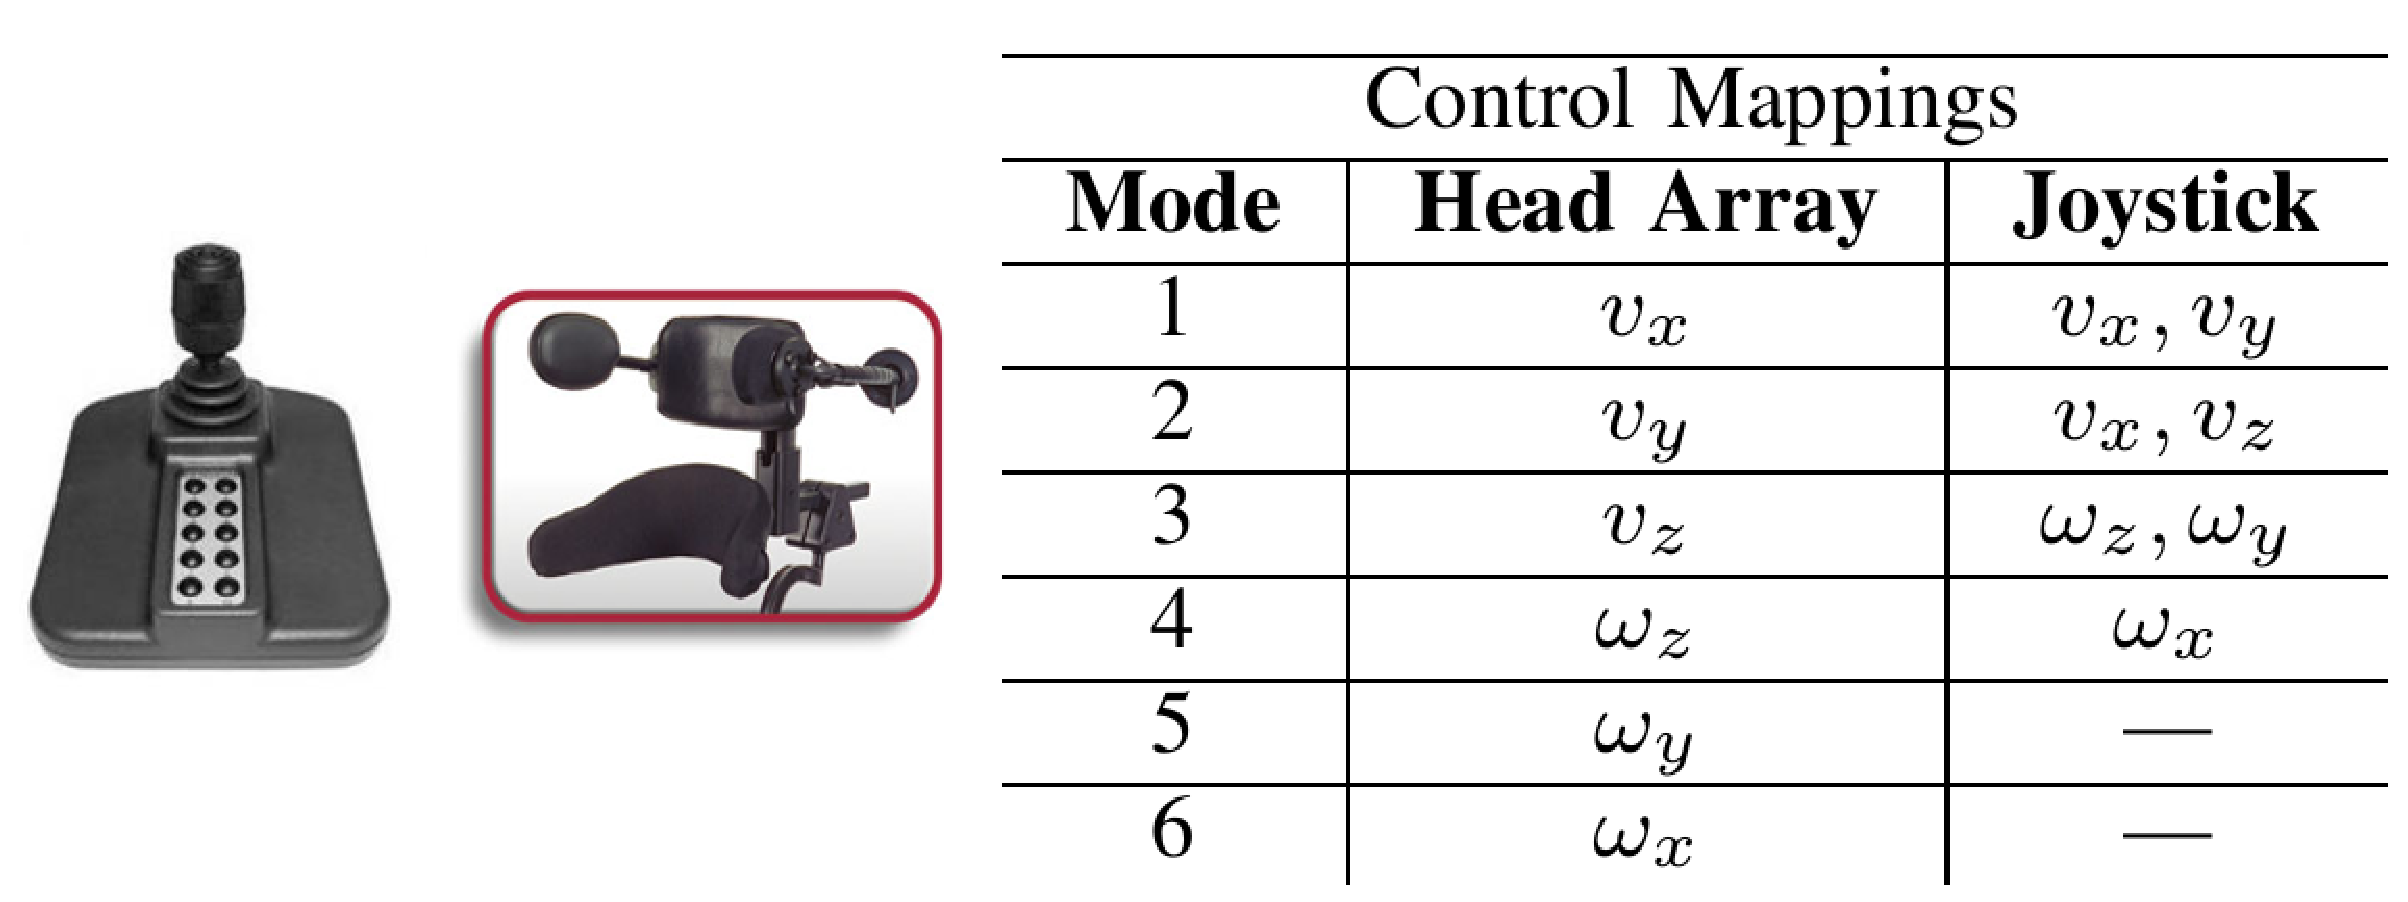
\includegraphics[width = 1\hsize, height = 0.14\vsize]{./figures/INTER_4.eps}
%	\vspace{-0.35cm}
	\caption{A 2-axis joystick (left) and switch-based head array (center) and their operational paradigms (right). $v$ and $\omega$ indicate the translational and rotational velocities of the end-effector, respectively.}
	\label{fig:interfaces}
\end{figure}
The users teleoperated the robot using two different control interfaces: a 2-axis joystick and a switch-based head array. The control signals captured from the interfaces were mapped to the Cartesian velocities of the end-effector (Figure~\ref{fig:interfaces}).

The joystick generated continuous control signals and the two dimensional mapping allowed for control of a maximum of two dimensions at a time. The 6-D control space was partitioned into four control modes that could be accessed using the buttons on the interface. On the other hand, the switch-based head array consisted of three switches embedded in the headset operated by the head and generated 1-D discrete signals. The switch at the back of the headset was used to cycle between the different control modes and the switches on the left and right controlled the motion of the robot's end effector in the positive and negative directions along the dimension corresponding to the selected control mode. An external button was provided to request the mode switch assistance. For both control interfaces the gripper had a dedicated control mode. 
\begin{figure*}[ht!]
	\includegraphics[keepaspectratio, width = \textwidth ]{./figures/Task_New.eps}
	\caption{Study tasks performed by subjects. \textit{Left:} Single-step reaching task. \textit{Right:} Multi-step Pouring task. }
	\label{fig:tasks}
\end{figure*}

\subsubsection{Assistance Paradigms}
Two kinds of mode switching assistance paradigms were evaluated in the study. Note that the blending assistance was always active in for both paradigms. Under the blending paradigm, the amount of assistance was directly proportional to the robot's confidence in estimating intent. Therefore, if intent inference improved as a result of goal disambiguation, more assistance would be provided by the robot likely resulting in better task performance. All trials started in a randomized initial control mode and home position. 

\noindent\underline{\textit{Manual}}: During task execution the user performed all mode switches. 

\noindent\underline{\textit{Disambiguation}}: The user could request mode switch assistance at any time during task execution. Upon assistance request, the algorithm identified and switched the current control mode to the ``best mode'' $m^*$. The user was required to request assistance at least once during task execution.  
\subsection{Task Descriptions}


\textbf{Training:} The training period consisted of three phases and two different task configurations. The subjects used both interfaces to perform the training tasks and lasted a maximum of 30 minutes.	

\noindent\underline{\textit{Phase One}}: The subjects were asked to perform simple reaching motion towards a single goal in the scene. This phase was intended for the subjects to get familiarized with the control interface mappings and teleoperation of the robotic arm. 

\noindent\underline{\textit{Phase Two}}: In the second phase of training, the blending-based shared autonomy was introduced. The subjects experienced how the robot helped in task execution. The subjects were informed that the robot autonomy will be present for all trials during the rest of the experiment. 

\noindent\underline{\textit{Phase Three}}: For the third phase of the training, multiple objects were introduced in the scene. 
%The subject was informed that when there are multiple objects in the scene, the robot can step in and help only if it has a good idea of which object they are going for. 
Subjects were informed that the robot had the capability to pick a control mode that it thinks will help it figure out which goal they were going for and that the subject had the option to activate the robot to pick that control mode. 
 The subject was asked to activate this option no later than half way into a reaching trial. Furthermore, the subject was also required to move as much as s/he can in the control mode chosen by the robot and observe the effects of autonomy. 


\noindent\textbf{Testing:} Two different testing tasks were developed for our study. 

\noindent\underline{\textit{Single-step:}} The user operated the robotic arm using both control interfaces to reach one of five objects on the table with a predefined orientation as the robot provides assistance (Figure~\ref{fig:tasks}, Left). 

\noindent\underline{\textit{Multi-step:}} This was a multi-step pouring task. The robot was fitted with a cup with contents at the start of the trial. The user was required to pour the contents of the cup in one of the two containers and then place the cup down at one of the two specified locations with a specific orientation (Figure~\ref{fig:tasks}, Right). 

\subsection{Study Protocol and Metrics}
\noindent\textbf{Subjects:} For this study eight subjects were recruited (mean age: $31 \pm 11$, 3 males and 5 females). All participants gave their informed, signed consent to participate in the experiment, which was approved by Northwestern University's Institutional Review Board. 
\begin{figure*}[ht!]
	\centering
	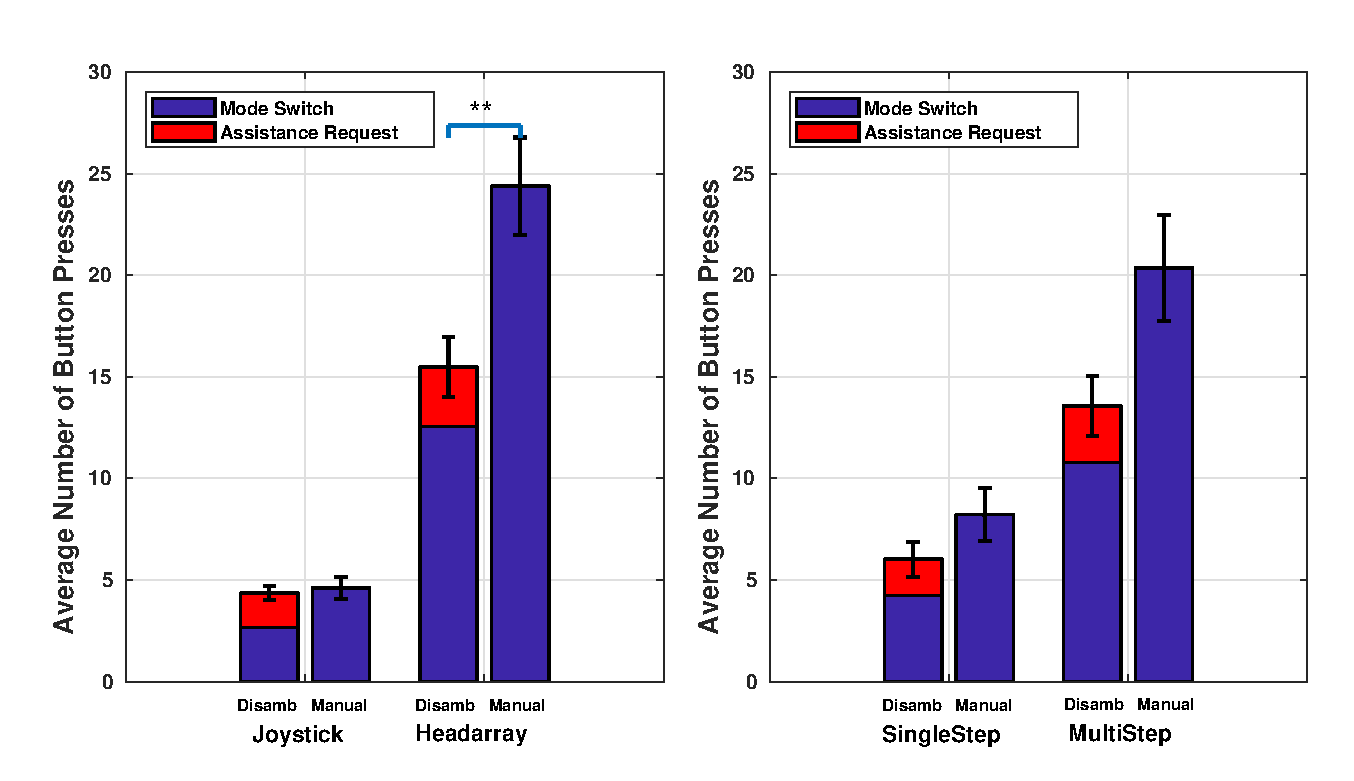
\includegraphics[keepaspectratio, width = 1\hsize ,center]{./figures/button_press_combined_shrunk.eps}
	\caption{Comparison of average number of button presses between \textit{Disambiguation} and \textit{Manual} Paradigms. \textit{Left:} Grouped by control interfaces. \textit{Right:} Grouped by tasks.}
	\label{fig:button_press}
\end{figure*}
\noindent\textbf{Protocol:}
A within-subjects study was conducted using a fractional factorial design in which the manipulated variables were the tasks, control interfaces and the assistance conditions. Each subject underwent an initial training period that lasted approximately thirty minutes after which the subject performed both tasks using both interfaces under the \textit{Manual} and \textit{Disambiguation} paradigms. The trials were balanced and the control interfaces and the paradigms were randomized and counterbalanced across all subjects to avoid ordering effects. Three trials were collected for the \textit{Manual} paradigm and five trials for the \textit{Disambiguation} paradigm. 

\noindent\textbf{Metrics:}
A number of objective metrics evaluated this study.  \textit{Number of mode switches} refer to the number of times a user switched between various control modes during task execution. \textit{Number of assistance requests} refer to the number of times user pressed the button requesting disambiguating assistance. \textit{Number of button presses} is the sum of \textit{Number of mode switches} and \textit{Number of assistance requests} and is also an indirect measure of the effort put forth by the user while accomplishing the task. We also characterize the temporal distribution of assistance requests.

%
%Comparision of confidence (mode of probability distibrution) pre/post assistance request. 
%Rate of mode switches pre/post assistance request. 
%Total number of mode switches
%Total time
%Timing of assistance request. Notion of difficulty and timing of mode switches and assistance request, correlation?
%Progress towards tasks pre/post assistance request. 


\section{Results}\label{sec:results}


Here we report the results of our subject study.  Statistical significance is determined by the Wilcoxon Rank-Sum test in Figure~\ref{fig:button_press} where (***) indicates $p < 0.001$, (**) $p < 0.01$ and (*) $p < 0.05$. 

\subsection{Impact of Disambiguation on Task Performance}
A statistically significant improvement in task performance in terms of a decrease in the number of button presses was observed between the \textit{Manual} and \textit{Disambiguation} paradigms when using the headarray (Figure~\ref{fig:button_press}, Left). Due to the low-dimensionality of headarray and cyclical nature of mode switching, the number of button presses required for task completion is inherently high. The disambiguation paradigm was helpful in reducing the number of button presses likely due to the fact that robot assistance was more effective in the disambiguating control mode and therefore reduced the need for subsequent user-initiated mode switches which in turn would have helped in reducing the task effort. For joystick, although statistically significant differences were observed for the number of mode switches between the two paradigms the gain due to the reduction of user-initiated mode switches was offset by the button presses that were required for assistance requests. 
A general trend (although not statistically significant) of a decrease in the number of button presses was also observed for the more complex multi-step task (Figure~\ref{fig:button_press}, Right). 
That is, subjects found most utility for the disambiguation paradigm when the control interface was more limited and the task was more complex.  
\begin{figure*}[ht!]
	\centering
	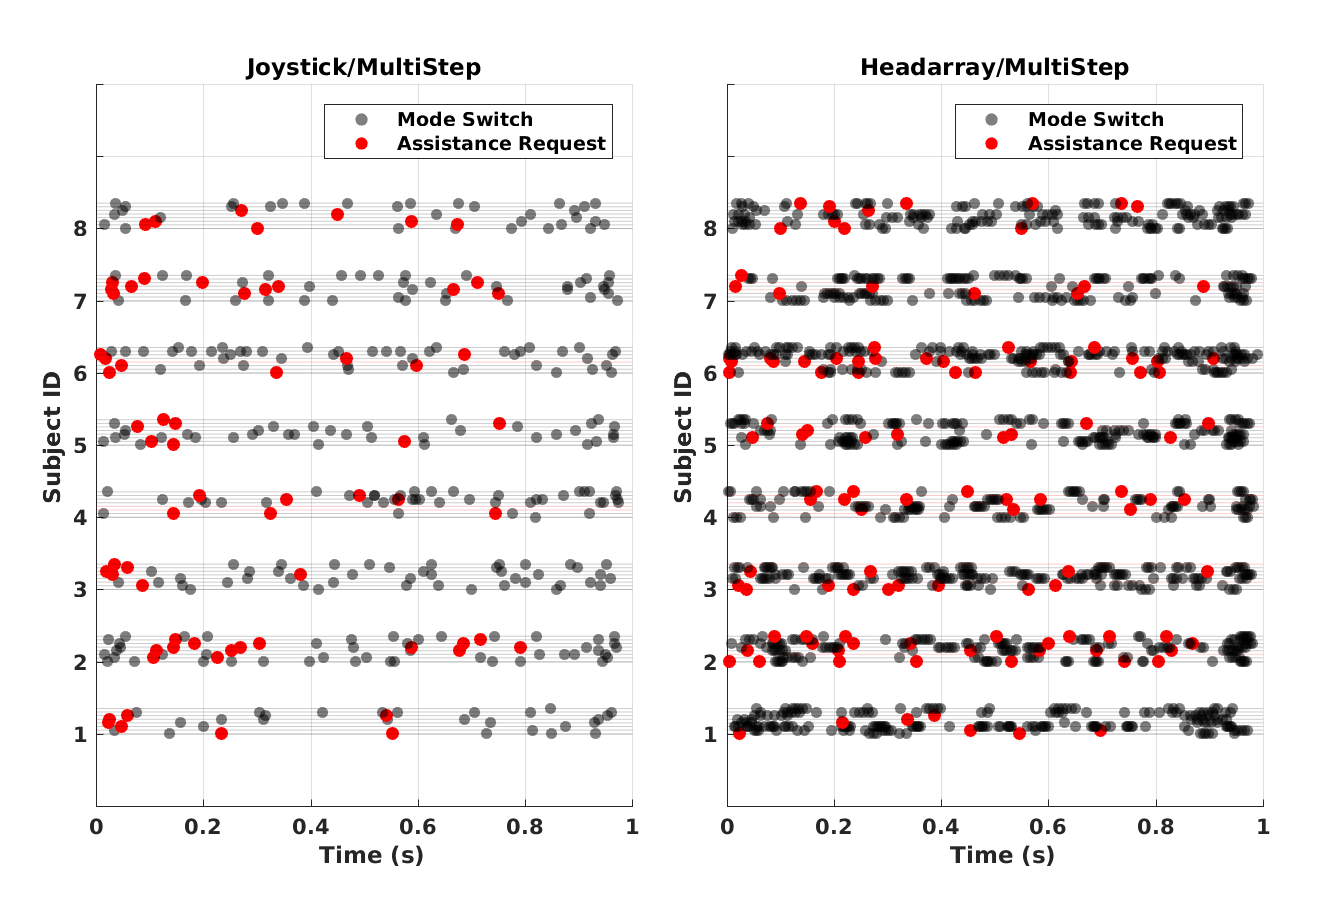
\includegraphics[ width = 0.9\textwidth, ,center]{./figures/j2_ha_man_disamb.eps}
	\caption{Temporal pattern of button presses for each interface/task combination on a trial-by-trial basis for all subjects. Eight trials per subject per interface/task combination. Gray and red horizontal lines denote successful and unsuccessful trials respectively.}
	\label{fig:ha_man_disamb}
\end{figure*}
\subsection{Temporal Distribution of Disambiguation Requests}
We also observed similar correlations between the \textit{temporal distribution} of disambiguation requests and the type of interface/task combinations. The temporal distribution of disambiguation requests refers to \textit{when} the subject requested assistance during the course of a trial. We use a measure of \textit{skewness} to characterize how much the temporal distribution deviates from a uniform distribution.\footnote{A uniform temporal distribution corresponds to a trial in which the assistance requests are uniformly spread out during the course of task execution. The skewness of a uniform distribution is $0$.} A positive value of skewness indicates that assistance requests are more concentrated to the earlier parts of the trials. Higher the skewness the more concentrated they are. Table~\ref{table:skewness} reports the skewness of the temporal distribution of assistance requests for different interface/task combinations. We observed that the assistance requests became more uniform (decreasing skewness values) as the interface/task combination became harder. The need for assistance is more persistent for these combinations and as a result the subjects would have utilized the disambiguation paradigm more evenly throughout the course of the trial. 
%\begin{figure*}[ht!]
%	%	\centering
%	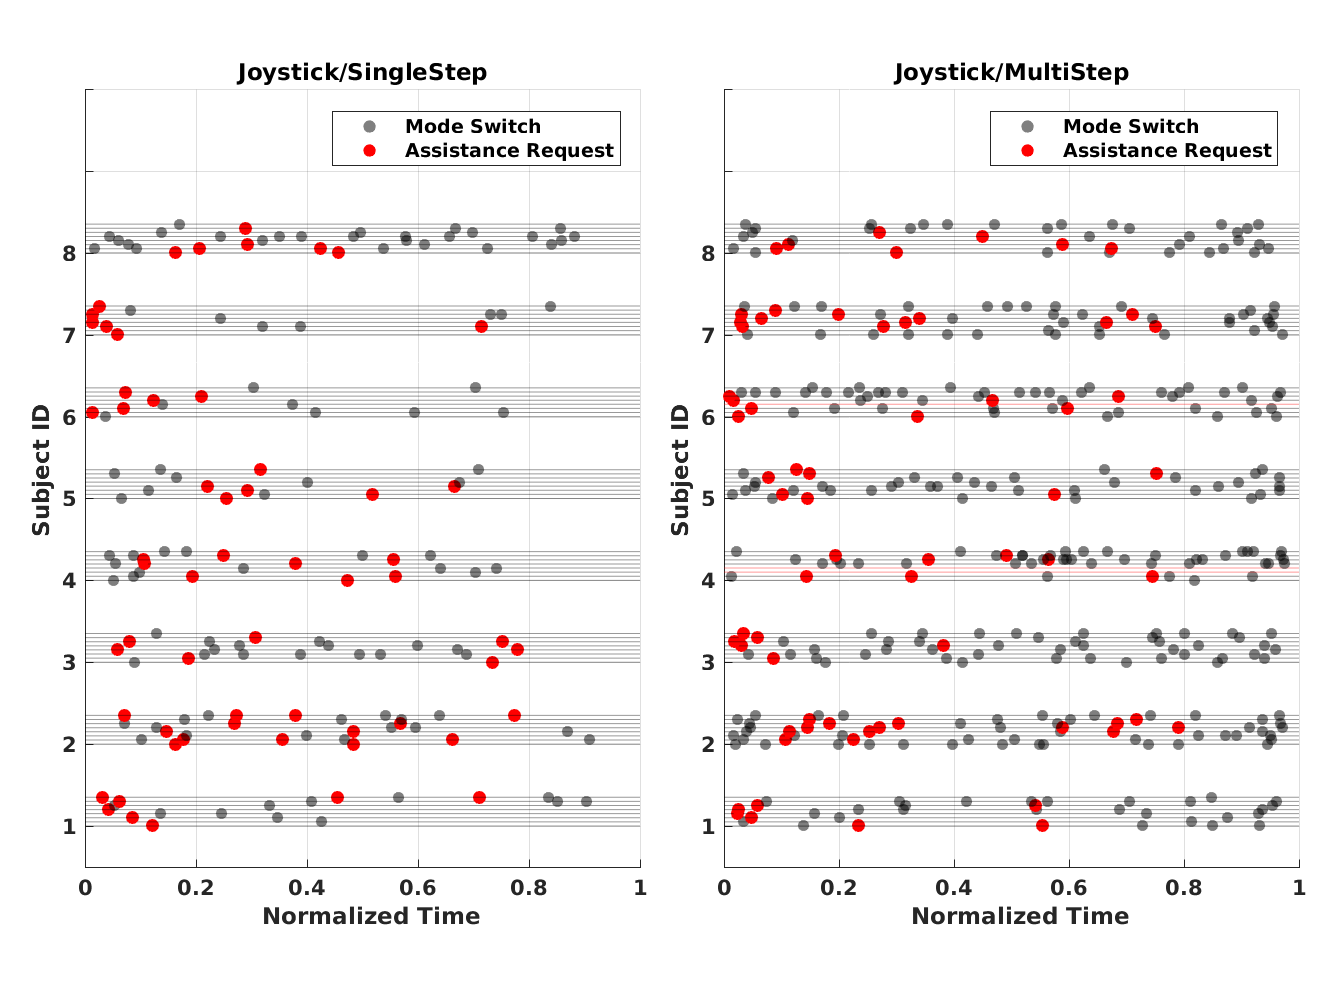
\includegraphics[ width = 0.9\textwidth, height=0.93\vsize ,center]{./figures/j2_man_disamb_pattern.eps}
%\end{figure*}


Figure~\ref{fig:ha_man_disamb} shows the temporal pattern for disambiguation requests and mode switches for the multi-step for both interfaces on a trial-by-trial basis for all subjects. From the figure it is clear that the frequency and density of button presses (both assistance requests and mode switches) are much higher for the more limited control interface. The subjects also demonstrated a diverse range of button press behavior. Some subjects preferred to perform manual mode switches to requesting assistance (e.g. Subject 1) whereas some others utilized the assistance paradigm a great deal more (e.g Subject 2). The variation between subjects is likely due to different factors such as the user's comfort in operating the robot and understanding the effectiveness of robot assistance in the disambiguating mode. 

\begin{table}[t]
	\centering
	\begin{tabular}{|c|c|c|c|}
		\hline
		& Single Step & Multi Step \\
		\hline
		Joystick & 0.63 & 0.57 \\
		\hline
		Headarray & 0.35 & 0.22 \\
		\hline
	\end{tabular}
	\vspace{.2cm}
	\caption{Characterization of the temporal distribution of assistance requests. The values in the table denotes the deviation of the temporal distribution from a uniform distribution. This deviation is captured using the \textit{Skewness} measure. } 
	\label{table:skewness}
	\vspace{-.5cm}
\end{table}

\begin{figure}[ht!]
	\centering
	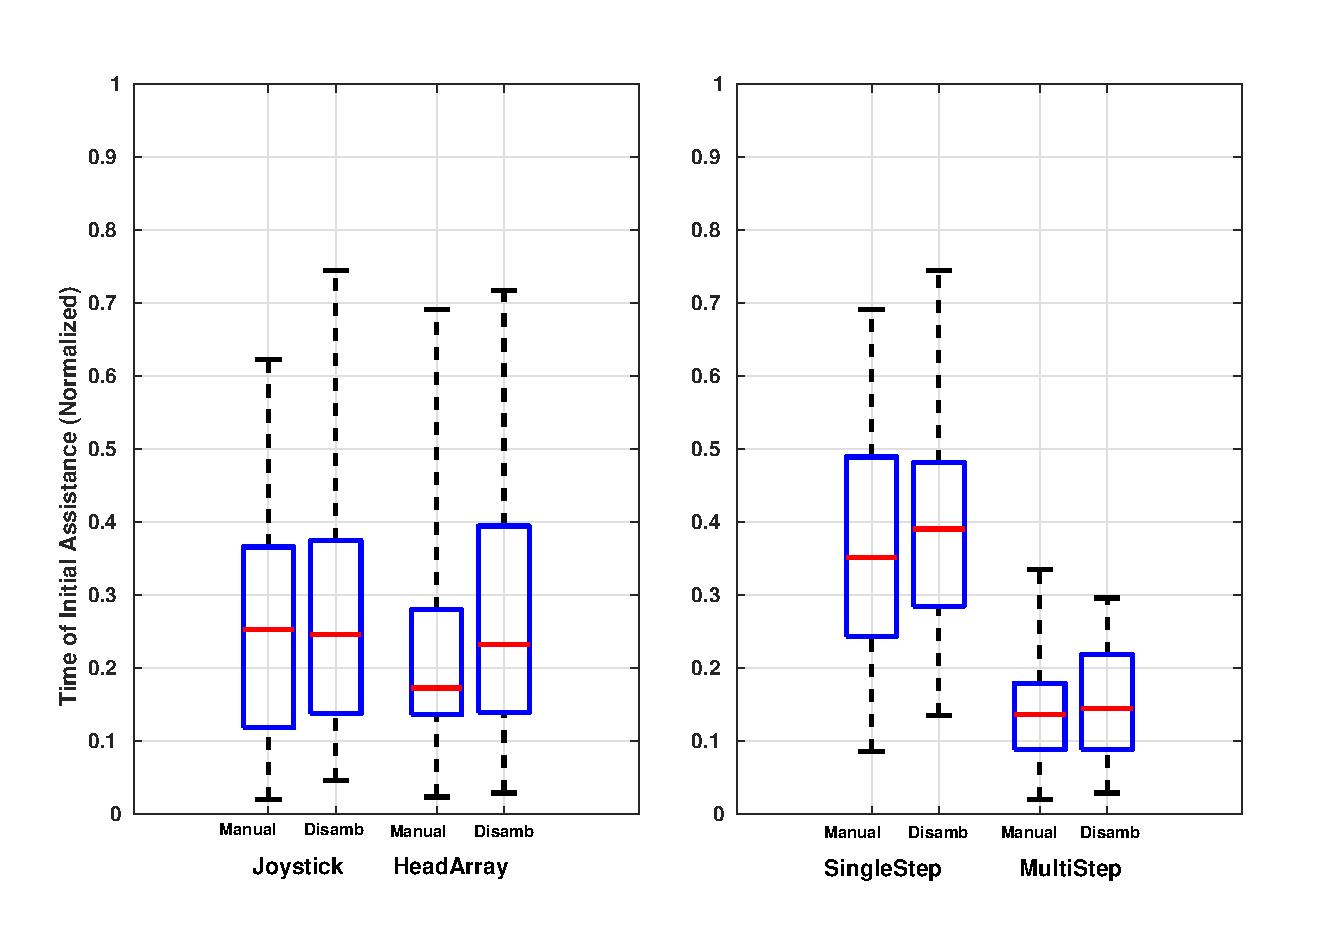
\includegraphics[width = 1\hsize ,center]{./figures/initial_blend_new.eps}
	\caption{Onset of robot assistance normalized with respect to task completion time. \textit{Left:} Across interfaces. \textit{Right:} Across tasks.}
	\label{fig:initial_blend}
\end{figure}
\subsection{Onset of Robot Assistance}\label{ssec:onset}
Our motivating intuition for developing the disambiguation system was that for disambiguation trials the robot assistance will step in earlier during the course of task execution. However, our results did not reveal any statistically significant differences between the two assistance paradigms across tasks and across interfaces (Figure~\ref{fig:initial_blend}). We think there are two plausible explanations for this. Firstly, subjects chose not to operate in the disambiguating modes and therefore did not `help' the robot in intent inference due to which the robot's confidence never passed the minimum threshold for assistance to step in. 
%\begin{figure}[ht!]
%	\centering
%	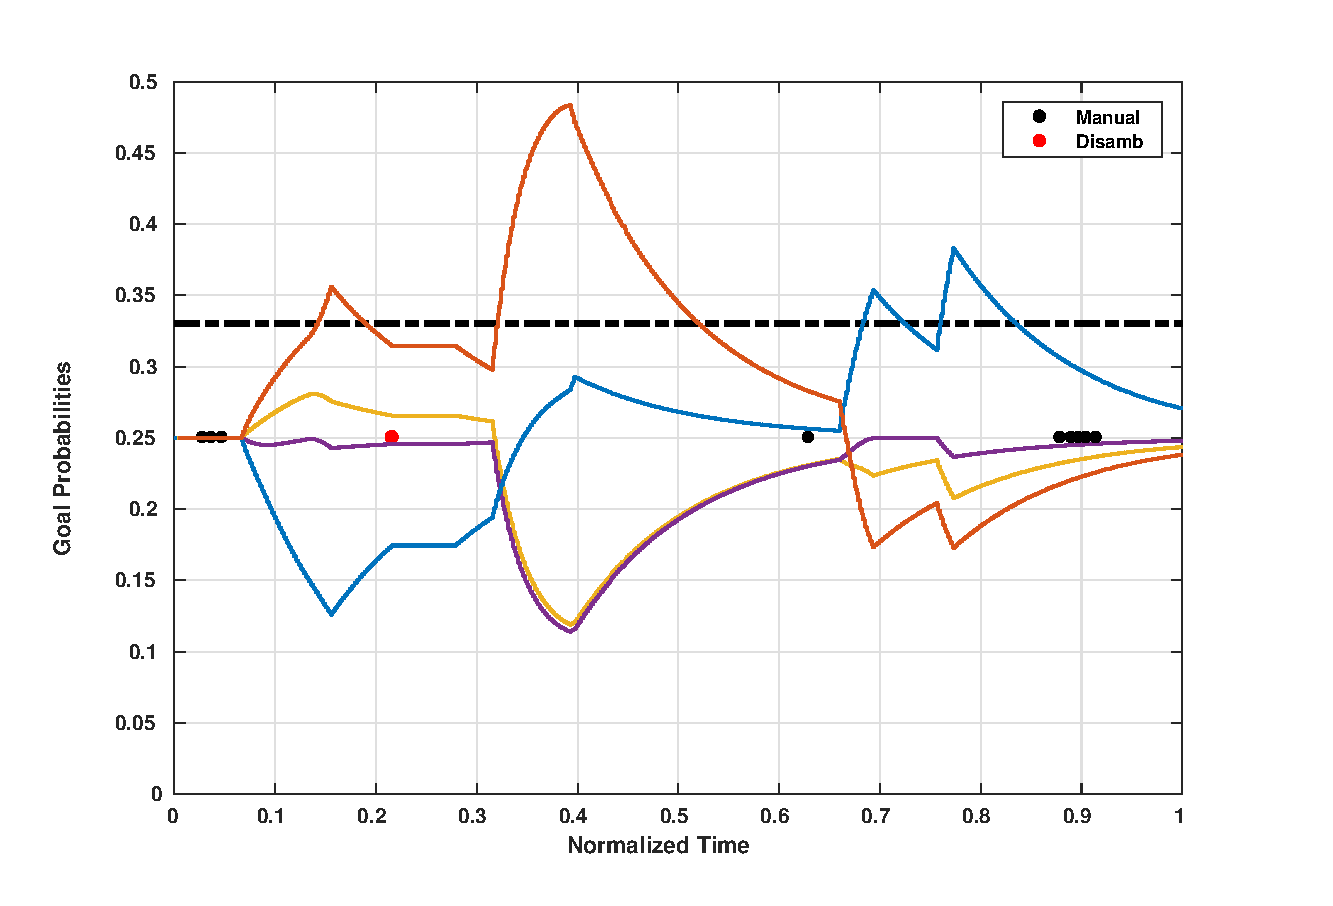
\includegraphics[width = 1.1\hsize ,center]{./figures/gp_ar_good.eps}
%\end{figure}

%\begin{figure}[ht!]
%	\centering
%	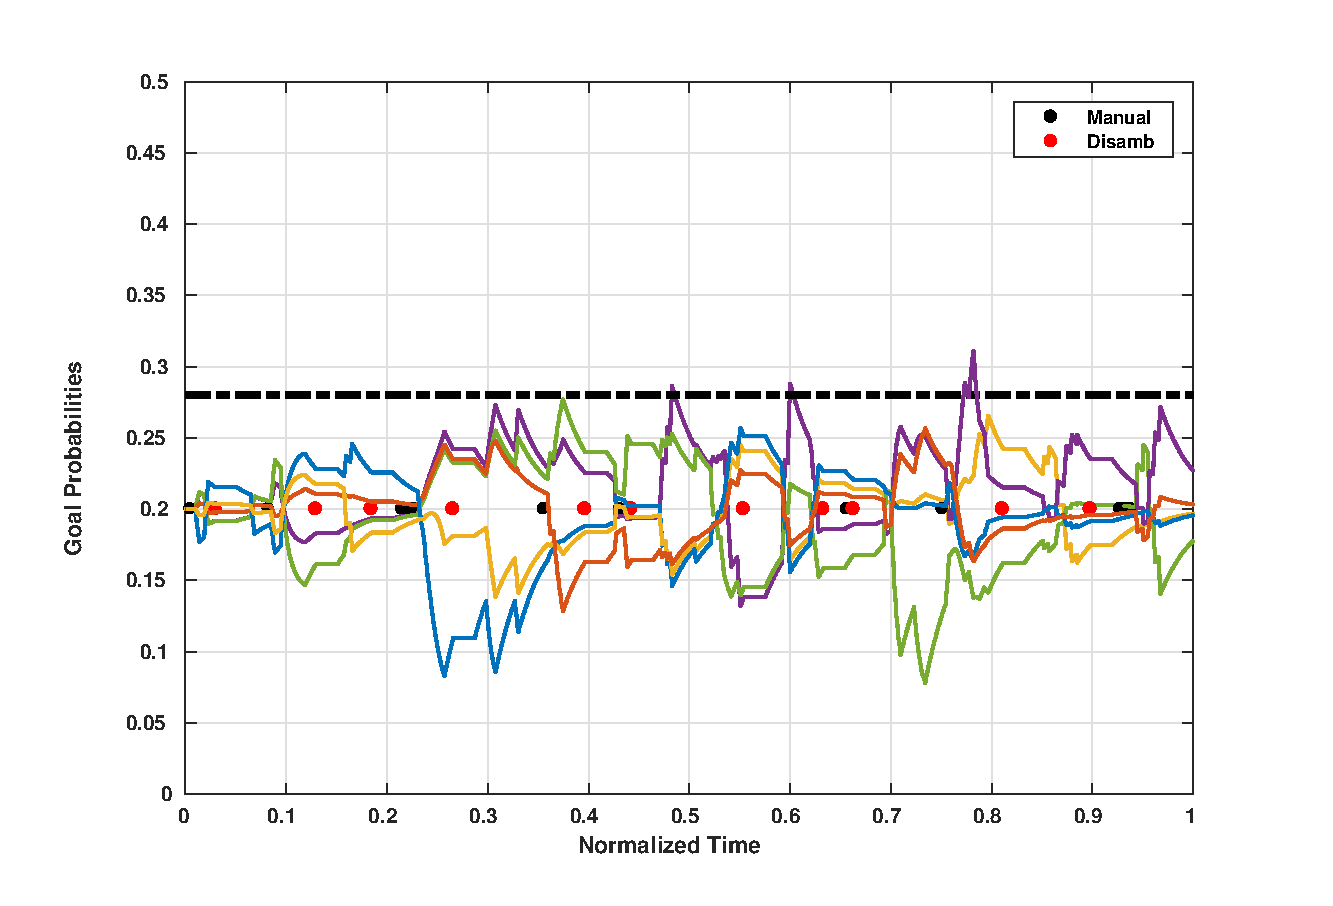
\includegraphics[width = 1.1\hsize ,center]{./figures/gp_ar_bad.eps}
%	\caption{Time evolution of goal probabilities. \textit{Top:} Subject A, Multi-step task. \textit{Bottom:} Subject B, Single-step task. The black horizontal line denotes the minimum threshold for robot assistance.}
%	\label{fig:gp_evolution}
%\end{figure}
Secondly, it was also possible that the training period was not sufficient enough for the subjects to gain a good grasp on what aspects of task execution did the robot rely on to provide assistance. Therefore, the subjects might not have had any incentive to operate in the disambiguating mode.
 
Figure~\ref{fig:gp_evolution} illustrates two very different approaches to performing the task and their impact on robot assistance. 
Subject A (Figure~\ref{fig:gp_evolution} (Top)) operated the robot in a more continuous fashion and chose to operate the robot in the disambiguating mode and thereby resulted in a sharp rise in goal confidence. On the other hand, Subject B operated the robot more sparsely and as a result the goal confidence did not cross the minimum threshold required for assistance. Despite the greater number of assistance requests, Subject B was not able to leverage the benefits of operating in a disambiguating mode and therefore the robot assistance was not able to step in earlier to help the user. 
\begin{figure}[ht!]
	\centering
	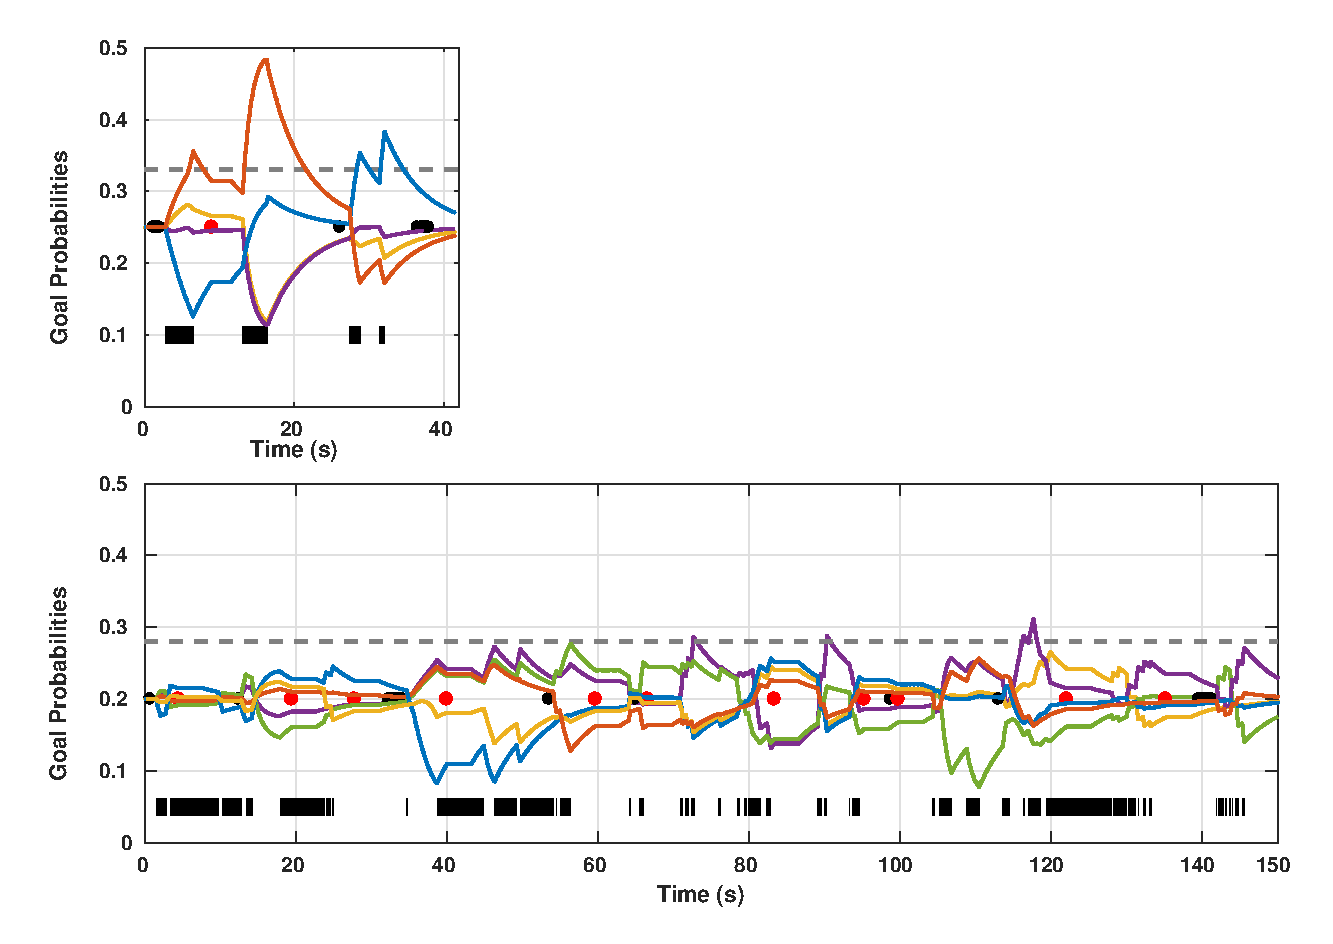
\includegraphics[width = 1\hsize, height=0.45\vsize, ,center]{./figures/gp_combined_with_line_gray.eps}
	\caption{Time evolution of goal probabilities. \textit{Top:} Multi-step task. \textit{Bottom:} Single-step task. The gray horizontal line above denotes the minimum threshold for robot assistance. The thick black line at the bottom denotes non-zero human control commands. The red and black dots indicate button presses that are assistance requests and mode switches respectively. }
	\label{fig:gp_evolution}
\end{figure}
%
\section{Discussion}\label{sec:discussions}
 
 
 In a \textit{help me, help you} type of human robot system, task execution becomes seamless and more efficient when there is a sound mutual understanding of how the other party operates. The robot uses its own intent inference engine to understand the human's intent. However, when subjects vary in responding to the training sessions, they also vary in their understanding of the robot's assistance. The knowledge of robot's assistance mechanism is paramount for the user to provide \textit{intent-expressive} control commands for the robot. 
 
 Therefore, the need for extensive and thorough training becomes apparent.
 The training can be made more effective in a few different ways---First, online feedback of the robot's intent prediction at all times during training can likely help the subject gain a better understanding of the relationship between the characteristics of their control actions (sparsity, aggressiveness, persistence) and the robot's assistive behavior. Second, the subjects could be explicitly informed of the task relevant features (directedness, proximity \textit{et cetera}) that the robot relies on for determining the amount of assistance. Knowledge of these features might motivate the users to leverage the advantages of operating the robot in the disambiguating mode. 
 
 The inherent time delays associated with the computation of the disambiguating mode (approximately 2-2.5s) might have been a discouraging factor and a cause for user frustration. The algorithm could be used to pre-compute a large set of most informative modes for different parts of the workspace, for different goal configurations and for different priors ahead of time, which then might be used a lookup table during task execution. Furthermore, metamodeling techniques and machine learning tools can be used to learn generalizable models that will be effective in previously unseen goal configurations. 
 
 In the present system, there is task effort associated with requesting assistance which can discourage the users from utilizing assistance. Automated mode switching schemes can possibly eliminate the need for button presses for assistance requests. 
 We also identify an opportunity to have adaptive assistance paradigms that explicitly take into account the characteristics of the user's control behavior. Some users are timid in their operation of the robot whereas some others are more aggressive and confident. Some are more comfortable operating the robot manually and do not seek assistance, whereas some others rely on assistance more frequently. Individual user characteristics could be extracted from the training data and be used for tuning the parameters of the intent inference engine and the shared control system to maximize robustness and efficacy of the assistive system. This would also likely improve user satisfaction and result in higher user acceptance. 
 
 
 
%Automated methods for triggering the computation of disambiguating mode can possibly results in savings in terms of button presses for assistance requests. Use metamodeling or machine learning techniques to generalize. Adaptive threshold for assistance that takes into account individual teleoperation characteristics. 
\section{Conclusion}\label{sec:conclusions}
In this paper, we have presented an algorithm for \textit{intent disambiguation assistance} with a shared-control robotic arm using the notion of \textit{inverse legibility}. The goal of this algorithm is to elicit more \textit{intent-expressive} control commands from the user by placing control in those control modes that \textit{maximally disambiguate} between the various goals in the scene. As a secondary contribution, we also present a novel intent inference mechanism inspired by \textit{dynamic field theory} that works in conjunction with the disambiguation system. A user study was conducted with eight subjects to evaluate the efficacy of the disambiguation system. Our results indicate a decrease in task effort in terms of the number of button presses when disambiguation system employed. 

%% For one-column wide figures use
%\begin{figure}
%% Use the relevant command to insert your figure file.
%% For example, with the graphicx package use
%  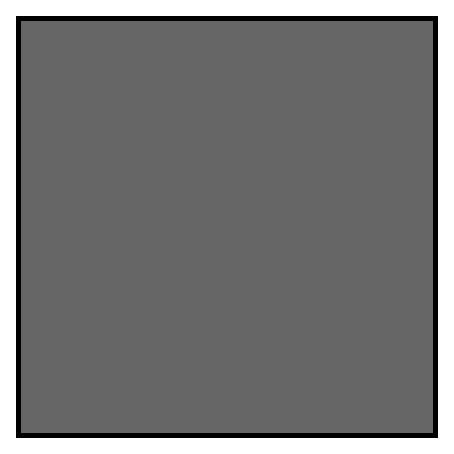
\includegraphics{example.eps}
%% figure caption is below the figure
%\caption{Figure1}
%\label{fig:1}       % Give a unique label
%\end{figure}
%%
%% For two-column wide figures use
%\begin{figure*}
%% Use the relevant command to insert your figure file.
%% For example, with the graphicx package use
%  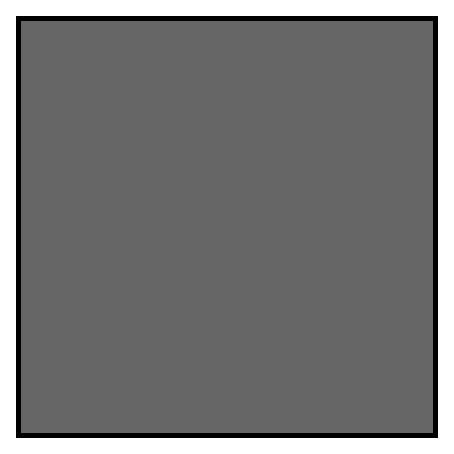
\includegraphics[width=0.75\textwidth]{example.eps}
%% figure caption is below the figure
%\caption{Figure2}
%\label{fig:2}       % Give a unique label
%\end{figure*}
%%
%% For tables use
%\begin{table}[h!]
%% table caption is above the table
%\caption{Please write your table caption here}
%\label{tab:1}       % Give a unique label
%% For LaTeX tables use
%\begin{tabular}{lll}
%\hline\noalign{\smallskip}
%first & second & third  \\
%\noalign{\smallskip}\hline\noalign{\smallskip}
%number & number & number \\
%number & number & number \\
%\noalign{\smallskip}\hline
%\end{tabular}
%\end{table}

% BibTeX users please use one of
\bibliographystyle{spbasic}      % basic style, author-year citations
%\bibliographystyle{spmpsci}      % mathematics and physical sciences
%\bibliographystyle{spphys}       % APS-like style for physics
\bibliography{references}   % name your BibTeX data base

% Non-BibTeX users please use
%\begin{thebibliography}{}
%%
%% and use \bibitem to create references. Consult the Instructions
%% for authors for reference list style.
%%
%\bibitem{RefJ}
%% Format for Journal Reference
%Author, Article title, Journal, Volume, page numbers (year)
%% Format for books
%\bibitem{RefB}
%Author, Book title, page numbers. Publisher, place (year)
%% etc
%\end{thebibliography}

\end{document}
% end of file template.tex

